% Capitolul 2: Distribuții clasice și fapte stilizate
% Statistica piețelor financiare -- Program de licență, Academia de Studii Economice din București
% GENERAT de latex/build_chapter2.py -- modificați generatorul, nu acest fișier.

\newcommand{\coursename}{Statistica piețelor financiare}
\def\sfmlang{ro}
% Preambul comun SFM -- Statistica piețelor financiare / Statistics of Financial Markets (Beamer, 16:9)
% Același design ca MFM. Înainte de % Preambul comun SFM -- Statistica piețelor financiare / Statistics of Financial Markets (Beamer, 16:9)
% Același design ca MFM. Înainte de % Preambul comun SFM -- Statistica piețelor financiare / Statistics of Financial Markets (Beamer, 16:9)
% Același design ca MFM. Înainte de \input{../../latex/preamble} se definește
%   \newcommand{\coursename}{Statistics of Financial Markets}      (EN)
%   \newcommand{\coursename}{Statistica piețelor financiare}       (RO)  și  \def\sfmlang{ro}
% Fișierele .tex se află în EN/Courses, EN/Seminars, RO/Cursuri, RO/Seminarii (două niveluri sub rădăcină).
% Deck-urile sînt generate de latex/build_chapterN.py / build_seminarN.py (vezi latex/sfm_build.py).

\documentclass[9pt, aspectratio=169, t]{beamer}
\providecommand{\coursename}{Statistics of Financial Markets}

% Ensure content fits on slides
\setbeamersize{text margin left=8mm, text margin right=8mm}

%=============================================================================
% THEME AND STYLE CONFIGURATION
%=============================================================================
\usetheme{default}
% Using default theme for clean header/footer control

% Color Palette (matching Redispatch PDF)
\definecolor{MainBlue}{RGB}{26, 58, 110}
\definecolor{AccentBlue}{RGB}{26, 58, 110}
\definecolor{IDAred}{RGB}{205, 0, 0}
\definecolor{DarkGray}{RGB}{51, 51, 51}
\definecolor{MediumGray}{RGB}{128, 128, 128}
\definecolor{LightGray}{RGB}{248, 248, 248}
\definecolor{VeryLightGray}{RGB}{235, 235, 235}
\definecolor{KeynoteGray}{RGB}{218, 218, 218}
\definecolor{SectionGray}{RGB}{120, 120, 120}
\definecolor{FooterGray}{RGB}{100, 100, 100}
\definecolor{Crimson}{RGB}{220, 53, 69}
\definecolor{Forest}{RGB}{46, 125, 50}
\definecolor{Amber}{RGB}{181, 133, 63}
\definecolor{Orange}{RGB}{230, 126, 34}
\definecolor{Purple}{RGB}{142, 68, 173}

% Gradient background (exact Keynote 315° gradient: white to RGB 218,218,218)
\setbeamertemplate{background}{%
    \begin{tikzpicture}[remember picture, overlay]
        \shade[shading=axis, shading angle=315,
        top color=white, bottom color=KeynoteGray]
        (current page.south west) rectangle (current page.north east);
    \end{tikzpicture}%
}
% Fallback solid color for compatibility
\setbeamercolor{background canvas}{bg=}

\setbeamercolor{palette primary}{bg=MainBlue, fg=white}
\setbeamercolor{palette secondary}{bg=MainBlue!85, fg=white}
\setbeamercolor{palette tertiary}{bg=MainBlue!70, fg=white}
\setbeamercolor{structure}{fg=MainBlue}
\setbeamercolor{title}{fg=IDAred}
\setbeamercolor{frametitle}{fg=IDAred, bg=}
\setbeamercolor{block title}{bg=MainBlue, fg=white}
\setbeamercolor{block body}{bg=VeryLightGray, fg=DarkGray}
\setbeamercolor{block title alerted}{bg=Crimson, fg=white}
\setbeamercolor{block body alerted}{bg=Crimson!8, fg=DarkGray}
\setbeamercolor{block title example}{bg=Forest, fg=white}
\setbeamercolor{block body example}{bg=Forest!8, fg=DarkGray}
\setbeamercolor{item}{fg=MainBlue}

% Footer colors (override Madrid theme blue)
\setbeamercolor{author in head/foot}{fg=FooterGray, bg=}
\setbeamercolor{title in head/foot}{fg=FooterGray, bg=}
\setbeamercolor{date in head/foot}{fg=FooterGray, bg=}
\setbeamercolor{section in head/foot}{fg=FooterGray, bg=}
\setbeamercolor{subsection in head/foot}{fg=FooterGray, bg=}

% Bullet styles (apply everywhere including blocks)
\setbeamertemplate{itemize item}{\color{MainBlue}$\boxdot$}
\setbeamertemplate{itemize subitem}{\color{MainBlue}$\blacktriangleright$}
\setbeamertemplate{itemize subsubitem}{\color{MainBlue}\tiny$\bullet$}
\setbeamertemplate{itemize/enumerate body begin}{\normalsize}
\setbeamertemplate{itemize/enumerate subbody begin}{\normalsize}

% Item spacing - compact style
\setlength{\leftmargini}{10pt}       % Level 1: minimal indent
\setlength{\leftmarginii}{10pt}      % Level 2: minimal additional indent
% Compact list spacing (zero extra space before/after lists in blocks)
\makeatletter
\def\@listi{\leftmargin\leftmargini \topsep 0pt \parsep 0pt \itemsep 0pt}
\def\@listii{\leftmargin\leftmarginii \topsep 0pt \parsep 0pt \itemsep 0pt}
\makeatother

\setbeamertemplate{navigation symbols}{}

%=============================================================================
% CUSTOM HEADLINE
%=============================================================================
\setbeamertemplate{headline}{%
    \vskip10pt%
    \hbox to \paperwidth{%
        \hskip0.5cm%
        {\small\color{FooterGray}\renewcommand{\hyperlink}[2]{##2}\insertsectionhead}%
        \hfill%
        \textcolor{FooterGray}{\small\insertframenumber}%
        \hskip0.5cm%
    }%
    \vskip4pt%
    {\color{FooterGray}\hrule height 0.4pt}%
}

%=============================================================================
% CUSTOM FOOTER
%=============================================================================
\usepackage{fontawesome5}

\setbeamertemplate{footline}{%
    {\color{FooterGray}\hrule height 0.4pt}%
    \vskip4pt%
    \hbox to \paperwidth{%
        \hskip0.5cm%
        \textcolor{FooterGray}{\small\coursename}%
        \hfill%
        \raisebox{-0.1em}{%
            \begin{tikzpicture}[x=0.08em, y=0.08em, line width=0.4pt]
                \draw[FooterGray] (0,3) -- (1,4) -- (2,3.5) -- (3,5) -- (4,4) -- (5,6) -- (6,5.5) -- (7,4) -- (8,5) -- (9,7) -- (10,6) -- (11,5) -- (12,6.5) -- (13,8) -- (14,7) -- (15,6) -- (16,7.5) -- (17,9) -- (18,8) -- (19,7) -- (20,8.5) -- (21,10) -- (22,9) -- (23,8) -- (24,9.5);
            \end{tikzpicture}%
        }%
        \hskip0.5cm%
    }%
    \vskip6pt%
}

%=============================================================================
% PACKAGES
%=============================================================================
\usepackage[utf8]{inputenc}
\DeclareUnicodeCharacter{03B1}{\ensuremath{\alpha}}
\usepackage[T1]{fontenc}
\usepackage{amsmath, amssymb, amsthm}
\usepackage{mathtools}
\usepackage{bm}
\usepackage{tikz}
\usetikzlibrary{arrows.meta, positioning, shapes, calc, decorations.pathreplacing, shadings}
\usepackage{booktabs}
\usepackage{multirow}
\usepackage{array}
\usepackage{graphicx}
\usepackage{hyperref}
\usepackage{colortbl}
\usepackage{listings}
\lstset{language=Python, basicstyle=\ttfamily\scriptsize, keywordstyle=\color{MainBlue}\bfseries,
  commentstyle=\color{Forest}, stringstyle=\color{Crimson}, breaklines=true,
  frame=none, backgroundcolor=\color{VeryLightGray}, xleftmargin=2mm}
\hypersetup{colorlinks=true, linkcolor=MainBlue, urlcolor=MainBlue}
\graphicspath{{../../logos/}{../../charts/}{../../photos/}}
\usepackage{xcolor}
\hfuzz=2pt  % Suppress tiny overfull warnings (<2pt)
\vfuzz=2pt  % Suppress tiny vertical overfull warnings (<2pt)

%=============================================================================
% QUANTLET COMMANDS
%   \quantlet{<displayed name>}{<url>}       (generic, compatible with the older SFM decks)
%   \sfmquantlet{Ch_05}{SFM_ch5_garch}       -> https://github.com/danpele/SFM/tree/main/Quantlets/Ch_05/SFM_ch5_garch
%   \qlurl{<folder>} is defined per chapter by the generator (Quantlets/Ch_NN/<folder>)
%=============================================================================
\newcommand{\sfmrepo}{https://github.com/danpele/SFM}
\newcommand{\sfmqlbase}{https://github.com/danpele/SFM/tree/main/Quantlets}
\newcommand{\quantlet}[2]{%
    \hfill\href{#2}{%
        \raisebox{-0.15em}{
\includegraphics[height=0.7em]{ql_logo.png}}%
        \textcolor{MainBlue}{\tiny\ #1}%
    }%
}
\newcommand{\sfmquantlet}[2]{\quantlet{\detokenize{#2}}{\sfmqlbase/#1/#2}}

%=============================================================================
% NOTEBOOKS (Google Colab)
%   \colaburl{notebooks/EN/chapter5_seminar_notebook.ipynb} -> the Colab link of a file in the SFM repo
%   \nb: the chapter notebook (each seminar deck redefines it with \renewcommand)
%=============================================================================
\newcommand{\colaburl}[1]{https://colab.research.google.com/github/danpele/SFM/blob/main/#1}
\newcommand{\nb}{https://colab.research.google.com/github/danpele/SFM/tree/main/notebooks/EN}
\newcommand{\nbname}{notebooks/EN}

%=============================================================================
% SLIDE HELPERS (used by the generators; the same as in MFM)
%=============================================================================
% local font size for list bodies (the preamble forces \normalsize)
\newcommand{\itemsize}[1]{\setbeamertemplate{itemize/enumerate body begin}{#1}\setbeamertemplate{itemize/enumerate subbody begin}{#1}}
\newcommand{\intitle}[1]{{\hypersetup{urlcolor=white}#1}}   % white links inside coloured title bars
\newcommand{\imgcap}[1]{{\scriptsize #1}\\[0.5mm]}          % caption under a photo
\newcommand{\imgcredit}[2]{{\tiny\color{FooterGray}\href{#1}{#2}}}   % image credit: source URL, author/licence
\newcommand{\aiprompt}[1]{{\ttfamily\color{MainBlue}#1}}     % a prompt to an AI assistant

%=============================================================================
% SEMINARS: student version by default; the instructor wrapper *_solutions.tex sets \solutionstrue
%=============================================================================
\makeatletter\@ifundefined{ifsolutions}{\expandafter\newif\csname ifsolutions\endcsname}{}\makeatother
\newcommand{\solonly}[1]{\ifsolutions #1\fi}
\newcommand{\propsub}{\ifsolutions\else\framesubtitle{\ifdefined\sfmlang Rezolvarea se discută la seminar\else Solution discussed in class\fi}\fi}

%=============================================================================
% APPENDIX AND CHAPTER LINKS (latex/appendix_links.py writes the calls; it also re-declares these
% macros before \begin{document}, so the decks compile with or without this preamble block)
%=============================================================================
\providecommand{\sfmapplink}[3]{\hypertarget{#2}{}\hyperlink{#1}{\beamergotobutton{#3}}}
\providecommand{\sfmappback}[2]{\begin{tikzpicture}[remember picture,overlay]\node[anchor=south east] at ([xshift=-3mm,yshift=7mm]current page.south east){\hyperlink{#1}{\beamerreturnbutton{#2}}};\end{tikzpicture}}
\providecommand{\sfmchlink}[2]{\href{#1}{#2}}
\providecommand{\sfmchlinkt}[2]{\href{#1}{\usebeamercolor[fg]{frametitle}#2}}

%=============================================================================
% QUANTINAR COMMAND: link către un curs Quantinar (subiecte avansate)
%=============================================================================
\newcommand{\quantinar}[2]{%
    \href{#2}{%
        \raisebox{-0.15em}{
\includegraphics[height=0.8em]{qr_logo.png}}%
        \textcolor{MainBlue}{\scriptsize\ #1}%
    }%
}

%=============================================================================
% CUSTOM TITLE PAGE
%=============================================================================
\defbeamertemplate*{title page}{hybrid}[1][]
{
    \vspace{0.2cm}
    % Logos row - top header (with clickable links)
    \begin{center}
        \href{https://www.ase.ro}{
\includegraphics[height=1.0cm]{ase_logo.png}}\hspace{0.3cm}%
        \href{https://theida.net}{
\includegraphics[height=1.0cm]{ida_logo.png}}\hspace{0.3cm}%
        \href{https://blockchain-research-center.com}{
\includegraphics[height=1.0cm]{brc_logo.png}}\hspace{0.3cm}%
        \href{https://www.ai4efin.ase.ro}{
\includegraphics[height=1.0cm]{ai4efin_logo.png}}\hspace{0.3cm}%
        \href{https://ipe.ro/new}{
\includegraphics[height=1.0cm]{acad_logo.png}}\hspace{0.3cm}%
        \href{https://www.digital-finance-msca.com}{
\includegraphics[height=1.0cm]{msca_logo.png}}%
    \end{center}

    \vspace{0.6cm}

    % Main title with Q logos on sides (with clickable links)
    \begin{center}
        \begin{minipage}{0.1\textwidth}
            \centering
            \href{https://quantlet.com}{
\includegraphics[height=1.1cm]{ql_logo.png}}
        \end{minipage}%
        \begin{minipage}{0.78\textwidth}
            \centering
            {\LARGE\bfseries\usebeamercolor[fg]{title}\inserttitle}

            \vspace{0.3cm}

            {\usebeamerfont{subtitle}\usebeamercolor[fg]{title}\insertsubtitle}
        \end{minipage}%
        \begin{minipage}{0.1\textwidth}
            \centering
            \href{https://quantinar.com}{
\includegraphics[height=1.1cm]{qr_logo.png}}
        \end{minipage}
    \end{center}

    \vspace{0.6cm}

    % Authors (left aligned)
    \hspace{0.5cm}{\usebeamerfont{author}\insertauthor}

    \vspace{0.3cm}

    % Institute/Affiliations (left aligned)
    \hspace{0.5cm}\begin{minipage}[t]{0.9\textwidth}
        \raggedright\small\insertinstitute
    \end{minipage}
}

%=============================================================================
% THEOREM ENVIRONMENTS
%=============================================================================
\theoremstyle{definition}
\setbeamertemplate{theorems}[numbered]
\ifdefined\sfmlang
\newtheorem{defn}{Definiție}
\newtheorem{thm}{Teoremă}
\newtheorem{prop}{Propoziție}
\newtheorem{rmk}{Observație}
\else
\newtheorem{defn}{Definition}
\newtheorem{thm}{Theorem}
\newtheorem{prop}{Proposition}
\newtheorem{rmk}{Remark}
\fi

%=============================================================================
% CENTRED MINIPAGE (no extra vertical space)
%=============================================================================
\newenvironment{cminipage}[1]{%
    \par\noindent\hfill\begin{minipage}{#1}\ignorespaces
}{%
    \end{minipage}\hfill\null\par
}

%=============================================================================
% CUSTOM COMMANDS
%=============================================================================
\newcommand{\E}{\mathbb{E}}
\newcommand{\Var}{\text{Var}}
\newcommand{\Cov}{\text{Cov}}
\newcommand{\Corr}{\text{Corr}}
\newcommand{\R}{\mathbb{R}}
\newcommand{\N}{\mathbb{N}}
\newcommand{\Z}{\mathbb{Z}}
\newcommand{\B}{\mathbf{B}}
\newcommand{\imark}{\textcolor{MainBlue}{\textbullet}}
\newcommand{\RMSE}{\text{RMSE}}
\newcommand{\MAE}{\text{MAE}}
\newcommand{\MAPE}{\text{MAPE}}

 se definește
%   \newcommand{\coursename}{Statistics of Financial Markets}      (EN)
%   \newcommand{\coursename}{Statistica piețelor financiare}       (RO)  și  \def\sfmlang{ro}
% Fișierele .tex se află în EN/Courses, EN/Seminars, RO/Cursuri, RO/Seminarii (două niveluri sub rădăcină).
% Deck-urile sînt generate de latex/build_chapterN.py / build_seminarN.py (vezi latex/sfm_build.py).

\documentclass[9pt, aspectratio=169, t]{beamer}
\providecommand{\coursename}{Statistics of Financial Markets}

% Ensure content fits on slides
\setbeamersize{text margin left=8mm, text margin right=8mm}

%=============================================================================
% THEME AND STYLE CONFIGURATION
%=============================================================================
\usetheme{default}
% Using default theme for clean header/footer control

% Color Palette (matching Redispatch PDF)
\definecolor{MainBlue}{RGB}{26, 58, 110}
\definecolor{AccentBlue}{RGB}{26, 58, 110}
\definecolor{IDAred}{RGB}{205, 0, 0}
\definecolor{DarkGray}{RGB}{51, 51, 51}
\definecolor{MediumGray}{RGB}{128, 128, 128}
\definecolor{LightGray}{RGB}{248, 248, 248}
\definecolor{VeryLightGray}{RGB}{235, 235, 235}
\definecolor{KeynoteGray}{RGB}{218, 218, 218}
\definecolor{SectionGray}{RGB}{120, 120, 120}
\definecolor{FooterGray}{RGB}{100, 100, 100}
\definecolor{Crimson}{RGB}{220, 53, 69}
\definecolor{Forest}{RGB}{46, 125, 50}
\definecolor{Amber}{RGB}{181, 133, 63}
\definecolor{Orange}{RGB}{230, 126, 34}
\definecolor{Purple}{RGB}{142, 68, 173}

% Gradient background (exact Keynote 315° gradient: white to RGB 218,218,218)
\setbeamertemplate{background}{%
    \begin{tikzpicture}[remember picture, overlay]
        \shade[shading=axis, shading angle=315,
        top color=white, bottom color=KeynoteGray]
        (current page.south west) rectangle (current page.north east);
    \end{tikzpicture}%
}
% Fallback solid color for compatibility
\setbeamercolor{background canvas}{bg=}

\setbeamercolor{palette primary}{bg=MainBlue, fg=white}
\setbeamercolor{palette secondary}{bg=MainBlue!85, fg=white}
\setbeamercolor{palette tertiary}{bg=MainBlue!70, fg=white}
\setbeamercolor{structure}{fg=MainBlue}
\setbeamercolor{title}{fg=IDAred}
\setbeamercolor{frametitle}{fg=IDAred, bg=}
\setbeamercolor{block title}{bg=MainBlue, fg=white}
\setbeamercolor{block body}{bg=VeryLightGray, fg=DarkGray}
\setbeamercolor{block title alerted}{bg=Crimson, fg=white}
\setbeamercolor{block body alerted}{bg=Crimson!8, fg=DarkGray}
\setbeamercolor{block title example}{bg=Forest, fg=white}
\setbeamercolor{block body example}{bg=Forest!8, fg=DarkGray}
\setbeamercolor{item}{fg=MainBlue}

% Footer colors (override Madrid theme blue)
\setbeamercolor{author in head/foot}{fg=FooterGray, bg=}
\setbeamercolor{title in head/foot}{fg=FooterGray, bg=}
\setbeamercolor{date in head/foot}{fg=FooterGray, bg=}
\setbeamercolor{section in head/foot}{fg=FooterGray, bg=}
\setbeamercolor{subsection in head/foot}{fg=FooterGray, bg=}

% Bullet styles (apply everywhere including blocks)
\setbeamertemplate{itemize item}{\color{MainBlue}$\boxdot$}
\setbeamertemplate{itemize subitem}{\color{MainBlue}$\blacktriangleright$}
\setbeamertemplate{itemize subsubitem}{\color{MainBlue}\tiny$\bullet$}
\setbeamertemplate{itemize/enumerate body begin}{\normalsize}
\setbeamertemplate{itemize/enumerate subbody begin}{\normalsize}

% Item spacing - compact style
\setlength{\leftmargini}{10pt}       % Level 1: minimal indent
\setlength{\leftmarginii}{10pt}      % Level 2: minimal additional indent
% Compact list spacing (zero extra space before/after lists in blocks)
\makeatletter
\def\@listi{\leftmargin\leftmargini \topsep 0pt \parsep 0pt \itemsep 0pt}
\def\@listii{\leftmargin\leftmarginii \topsep 0pt \parsep 0pt \itemsep 0pt}
\makeatother

\setbeamertemplate{navigation symbols}{}

%=============================================================================
% CUSTOM HEADLINE
%=============================================================================
\setbeamertemplate{headline}{%
    \vskip10pt%
    \hbox to \paperwidth{%
        \hskip0.5cm%
        {\small\color{FooterGray}\renewcommand{\hyperlink}[2]{##2}\insertsectionhead}%
        \hfill%
        \textcolor{FooterGray}{\small\insertframenumber}%
        \hskip0.5cm%
    }%
    \vskip4pt%
    {\color{FooterGray}\hrule height 0.4pt}%
}

%=============================================================================
% CUSTOM FOOTER
%=============================================================================
\usepackage{fontawesome5}

\setbeamertemplate{footline}{%
    {\color{FooterGray}\hrule height 0.4pt}%
    \vskip4pt%
    \hbox to \paperwidth{%
        \hskip0.5cm%
        \textcolor{FooterGray}{\small\coursename}%
        \hfill%
        \raisebox{-0.1em}{%
            \begin{tikzpicture}[x=0.08em, y=0.08em, line width=0.4pt]
                \draw[FooterGray] (0,3) -- (1,4) -- (2,3.5) -- (3,5) -- (4,4) -- (5,6) -- (6,5.5) -- (7,4) -- (8,5) -- (9,7) -- (10,6) -- (11,5) -- (12,6.5) -- (13,8) -- (14,7) -- (15,6) -- (16,7.5) -- (17,9) -- (18,8) -- (19,7) -- (20,8.5) -- (21,10) -- (22,9) -- (23,8) -- (24,9.5);
            \end{tikzpicture}%
        }%
        \hskip0.5cm%
    }%
    \vskip6pt%
}

%=============================================================================
% PACKAGES
%=============================================================================
\usepackage[utf8]{inputenc}
\DeclareUnicodeCharacter{03B1}{\ensuremath{\alpha}}
\usepackage[T1]{fontenc}
\usepackage{amsmath, amssymb, amsthm}
\usepackage{mathtools}
\usepackage{bm}
\usepackage{tikz}
\usetikzlibrary{arrows.meta, positioning, shapes, calc, decorations.pathreplacing, shadings}
\usepackage{booktabs}
\usepackage{multirow}
\usepackage{array}
\usepackage{graphicx}
\usepackage{hyperref}
\usepackage{colortbl}
\usepackage{listings}
\lstset{language=Python, basicstyle=\ttfamily\scriptsize, keywordstyle=\color{MainBlue}\bfseries,
  commentstyle=\color{Forest}, stringstyle=\color{Crimson}, breaklines=true,
  frame=none, backgroundcolor=\color{VeryLightGray}, xleftmargin=2mm}
\hypersetup{colorlinks=true, linkcolor=MainBlue, urlcolor=MainBlue}
\graphicspath{{../../logos/}{../../charts/}{../../photos/}}
\usepackage{xcolor}
\hfuzz=2pt  % Suppress tiny overfull warnings (<2pt)
\vfuzz=2pt  % Suppress tiny vertical overfull warnings (<2pt)

%=============================================================================
% QUANTLET COMMANDS
%   \quantlet{<displayed name>}{<url>}       (generic, compatible with the older SFM decks)
%   \sfmquantlet{Ch_05}{SFM_ch5_garch}       -> https://github.com/danpele/SFM/tree/main/Quantlets/Ch_05/SFM_ch5_garch
%   \qlurl{<folder>} is defined per chapter by the generator (Quantlets/Ch_NN/<folder>)
%=============================================================================
\newcommand{\sfmrepo}{https://github.com/danpele/SFM}
\newcommand{\sfmqlbase}{https://github.com/danpele/SFM/tree/main/Quantlets}
\newcommand{\quantlet}[2]{%
    \hfill\href{#2}{%
        \raisebox{-0.15em}{
\includegraphics[height=0.7em]{ql_logo.png}}%
        \textcolor{MainBlue}{\tiny\ #1}%
    }%
}
\newcommand{\sfmquantlet}[2]{\quantlet{\detokenize{#2}}{\sfmqlbase/#1/#2}}

%=============================================================================
% NOTEBOOKS (Google Colab)
%   \colaburl{notebooks/EN/chapter5_seminar_notebook.ipynb} -> the Colab link of a file in the SFM repo
%   \nb: the chapter notebook (each seminar deck redefines it with \renewcommand)
%=============================================================================
\newcommand{\colaburl}[1]{https://colab.research.google.com/github/danpele/SFM/blob/main/#1}
\newcommand{\nb}{https://colab.research.google.com/github/danpele/SFM/tree/main/notebooks/EN}
\newcommand{\nbname}{notebooks/EN}

%=============================================================================
% SLIDE HELPERS (used by the generators; the same as in MFM)
%=============================================================================
% local font size for list bodies (the preamble forces \normalsize)
\newcommand{\itemsize}[1]{\setbeamertemplate{itemize/enumerate body begin}{#1}\setbeamertemplate{itemize/enumerate subbody begin}{#1}}
\newcommand{\intitle}[1]{{\hypersetup{urlcolor=white}#1}}   % white links inside coloured title bars
\newcommand{\imgcap}[1]{{\scriptsize #1}\\[0.5mm]}          % caption under a photo
\newcommand{\imgcredit}[2]{{\tiny\color{FooterGray}\href{#1}{#2}}}   % image credit: source URL, author/licence
\newcommand{\aiprompt}[1]{{\ttfamily\color{MainBlue}#1}}     % a prompt to an AI assistant

%=============================================================================
% SEMINARS: student version by default; the instructor wrapper *_solutions.tex sets \solutionstrue
%=============================================================================
\makeatletter\@ifundefined{ifsolutions}{\expandafter\newif\csname ifsolutions\endcsname}{}\makeatother
\newcommand{\solonly}[1]{\ifsolutions #1\fi}
\newcommand{\propsub}{\ifsolutions\else\framesubtitle{\ifdefined\sfmlang Rezolvarea se discută la seminar\else Solution discussed in class\fi}\fi}

%=============================================================================
% APPENDIX AND CHAPTER LINKS (latex/appendix_links.py writes the calls; it also re-declares these
% macros before \begin{document}, so the decks compile with or without this preamble block)
%=============================================================================
\providecommand{\sfmapplink}[3]{\hypertarget{#2}{}\hyperlink{#1}{\beamergotobutton{#3}}}
\providecommand{\sfmappback}[2]{\begin{tikzpicture}[remember picture,overlay]\node[anchor=south east] at ([xshift=-3mm,yshift=7mm]current page.south east){\hyperlink{#1}{\beamerreturnbutton{#2}}};\end{tikzpicture}}
\providecommand{\sfmchlink}[2]{\href{#1}{#2}}
\providecommand{\sfmchlinkt}[2]{\href{#1}{\usebeamercolor[fg]{frametitle}#2}}

%=============================================================================
% QUANTINAR COMMAND: link către un curs Quantinar (subiecte avansate)
%=============================================================================
\newcommand{\quantinar}[2]{%
    \href{#2}{%
        \raisebox{-0.15em}{
\includegraphics[height=0.8em]{qr_logo.png}}%
        \textcolor{MainBlue}{\scriptsize\ #1}%
    }%
}

%=============================================================================
% CUSTOM TITLE PAGE
%=============================================================================
\defbeamertemplate*{title page}{hybrid}[1][]
{
    \vspace{0.2cm}
    % Logos row - top header (with clickable links)
    \begin{center}
        \href{https://www.ase.ro}{
\includegraphics[height=1.0cm]{ase_logo.png}}\hspace{0.3cm}%
        \href{https://theida.net}{
\includegraphics[height=1.0cm]{ida_logo.png}}\hspace{0.3cm}%
        \href{https://blockchain-research-center.com}{
\includegraphics[height=1.0cm]{brc_logo.png}}\hspace{0.3cm}%
        \href{https://www.ai4efin.ase.ro}{
\includegraphics[height=1.0cm]{ai4efin_logo.png}}\hspace{0.3cm}%
        \href{https://ipe.ro/new}{
\includegraphics[height=1.0cm]{acad_logo.png}}\hspace{0.3cm}%
        \href{https://www.digital-finance-msca.com}{
\includegraphics[height=1.0cm]{msca_logo.png}}%
    \end{center}

    \vspace{0.6cm}

    % Main title with Q logos on sides (with clickable links)
    \begin{center}
        \begin{minipage}{0.1\textwidth}
            \centering
            \href{https://quantlet.com}{
\includegraphics[height=1.1cm]{ql_logo.png}}
        \end{minipage}%
        \begin{minipage}{0.78\textwidth}
            \centering
            {\LARGE\bfseries\usebeamercolor[fg]{title}\inserttitle}

            \vspace{0.3cm}

            {\usebeamerfont{subtitle}\usebeamercolor[fg]{title}\insertsubtitle}
        \end{minipage}%
        \begin{minipage}{0.1\textwidth}
            \centering
            \href{https://quantinar.com}{
\includegraphics[height=1.1cm]{qr_logo.png}}
        \end{minipage}
    \end{center}

    \vspace{0.6cm}

    % Authors (left aligned)
    \hspace{0.5cm}{\usebeamerfont{author}\insertauthor}

    \vspace{0.3cm}

    % Institute/Affiliations (left aligned)
    \hspace{0.5cm}\begin{minipage}[t]{0.9\textwidth}
        \raggedright\small\insertinstitute
    \end{minipage}
}

%=============================================================================
% THEOREM ENVIRONMENTS
%=============================================================================
\theoremstyle{definition}
\setbeamertemplate{theorems}[numbered]
\ifdefined\sfmlang
\newtheorem{defn}{Definiție}
\newtheorem{thm}{Teoremă}
\newtheorem{prop}{Propoziție}
\newtheorem{rmk}{Observație}
\else
\newtheorem{defn}{Definition}
\newtheorem{thm}{Theorem}
\newtheorem{prop}{Proposition}
\newtheorem{rmk}{Remark}
\fi

%=============================================================================
% CENTRED MINIPAGE (no extra vertical space)
%=============================================================================
\newenvironment{cminipage}[1]{%
    \par\noindent\hfill\begin{minipage}{#1}\ignorespaces
}{%
    \end{minipage}\hfill\null\par
}

%=============================================================================
% CUSTOM COMMANDS
%=============================================================================
\newcommand{\E}{\mathbb{E}}
\newcommand{\Var}{\text{Var}}
\newcommand{\Cov}{\text{Cov}}
\newcommand{\Corr}{\text{Corr}}
\newcommand{\R}{\mathbb{R}}
\newcommand{\N}{\mathbb{N}}
\newcommand{\Z}{\mathbb{Z}}
\newcommand{\B}{\mathbf{B}}
\newcommand{\imark}{\textcolor{MainBlue}{\textbullet}}
\newcommand{\RMSE}{\text{RMSE}}
\newcommand{\MAE}{\text{MAE}}
\newcommand{\MAPE}{\text{MAPE}}

 se definește
%   \newcommand{\coursename}{Statistics of Financial Markets}      (EN)
%   \newcommand{\coursename}{Statistica piețelor financiare}       (RO)  și  \def\sfmlang{ro}
% Fișierele .tex se află în EN/Courses, EN/Seminars, RO/Cursuri, RO/Seminarii (două niveluri sub rădăcină).
% Deck-urile sînt generate de latex/build_chapterN.py / build_seminarN.py (vezi latex/sfm_build.py).

\documentclass[9pt, aspectratio=169, t]{beamer}
\providecommand{\coursename}{Statistics of Financial Markets}

% Ensure content fits on slides
\setbeamersize{text margin left=8mm, text margin right=8mm}

%=============================================================================
% THEME AND STYLE CONFIGURATION
%=============================================================================
\usetheme{default}
% Using default theme for clean header/footer control

% Color Palette (matching Redispatch PDF)
\definecolor{MainBlue}{RGB}{26, 58, 110}
\definecolor{AccentBlue}{RGB}{26, 58, 110}
\definecolor{IDAred}{RGB}{205, 0, 0}
\definecolor{DarkGray}{RGB}{51, 51, 51}
\definecolor{MediumGray}{RGB}{128, 128, 128}
\definecolor{LightGray}{RGB}{248, 248, 248}
\definecolor{VeryLightGray}{RGB}{235, 235, 235}
\definecolor{KeynoteGray}{RGB}{218, 218, 218}
\definecolor{SectionGray}{RGB}{120, 120, 120}
\definecolor{FooterGray}{RGB}{100, 100, 100}
\definecolor{Crimson}{RGB}{220, 53, 69}
\definecolor{Forest}{RGB}{46, 125, 50}
\definecolor{Amber}{RGB}{181, 133, 63}
\definecolor{Orange}{RGB}{230, 126, 34}
\definecolor{Purple}{RGB}{142, 68, 173}

% Gradient background (exact Keynote 315° gradient: white to RGB 218,218,218)
\setbeamertemplate{background}{%
    \begin{tikzpicture}[remember picture, overlay]
        \shade[shading=axis, shading angle=315,
        top color=white, bottom color=KeynoteGray]
        (current page.south west) rectangle (current page.north east);
    \end{tikzpicture}%
}
% Fallback solid color for compatibility
\setbeamercolor{background canvas}{bg=}

\setbeamercolor{palette primary}{bg=MainBlue, fg=white}
\setbeamercolor{palette secondary}{bg=MainBlue!85, fg=white}
\setbeamercolor{palette tertiary}{bg=MainBlue!70, fg=white}
\setbeamercolor{structure}{fg=MainBlue}
\setbeamercolor{title}{fg=IDAred}
\setbeamercolor{frametitle}{fg=IDAred, bg=}
\setbeamercolor{block title}{bg=MainBlue, fg=white}
\setbeamercolor{block body}{bg=VeryLightGray, fg=DarkGray}
\setbeamercolor{block title alerted}{bg=Crimson, fg=white}
\setbeamercolor{block body alerted}{bg=Crimson!8, fg=DarkGray}
\setbeamercolor{block title example}{bg=Forest, fg=white}
\setbeamercolor{block body example}{bg=Forest!8, fg=DarkGray}
\setbeamercolor{item}{fg=MainBlue}

% Footer colors (override Madrid theme blue)
\setbeamercolor{author in head/foot}{fg=FooterGray, bg=}
\setbeamercolor{title in head/foot}{fg=FooterGray, bg=}
\setbeamercolor{date in head/foot}{fg=FooterGray, bg=}
\setbeamercolor{section in head/foot}{fg=FooterGray, bg=}
\setbeamercolor{subsection in head/foot}{fg=FooterGray, bg=}

% Bullet styles (apply everywhere including blocks)
\setbeamertemplate{itemize item}{\color{MainBlue}$\boxdot$}
\setbeamertemplate{itemize subitem}{\color{MainBlue}$\blacktriangleright$}
\setbeamertemplate{itemize subsubitem}{\color{MainBlue}\tiny$\bullet$}
\setbeamertemplate{itemize/enumerate body begin}{\normalsize}
\setbeamertemplate{itemize/enumerate subbody begin}{\normalsize}

% Item spacing - compact style
\setlength{\leftmargini}{10pt}       % Level 1: minimal indent
\setlength{\leftmarginii}{10pt}      % Level 2: minimal additional indent
% Compact list spacing (zero extra space before/after lists in blocks)
\makeatletter
\def\@listi{\leftmargin\leftmargini \topsep 0pt \parsep 0pt \itemsep 0pt}
\def\@listii{\leftmargin\leftmarginii \topsep 0pt \parsep 0pt \itemsep 0pt}
\makeatother

\setbeamertemplate{navigation symbols}{}

%=============================================================================
% CUSTOM HEADLINE
%=============================================================================
\setbeamertemplate{headline}{%
    \vskip10pt%
    \hbox to \paperwidth{%
        \hskip0.5cm%
        {\small\color{FooterGray}\renewcommand{\hyperlink}[2]{##2}\insertsectionhead}%
        \hfill%
        \textcolor{FooterGray}{\small\insertframenumber}%
        \hskip0.5cm%
    }%
    \vskip4pt%
    {\color{FooterGray}\hrule height 0.4pt}%
}

%=============================================================================
% CUSTOM FOOTER
%=============================================================================
\usepackage{fontawesome5}

\setbeamertemplate{footline}{%
    {\color{FooterGray}\hrule height 0.4pt}%
    \vskip4pt%
    \hbox to \paperwidth{%
        \hskip0.5cm%
        \textcolor{FooterGray}{\small\coursename}%
        \hfill%
        \raisebox{-0.1em}{%
            \begin{tikzpicture}[x=0.08em, y=0.08em, line width=0.4pt]
                \draw[FooterGray] (0,3) -- (1,4) -- (2,3.5) -- (3,5) -- (4,4) -- (5,6) -- (6,5.5) -- (7,4) -- (8,5) -- (9,7) -- (10,6) -- (11,5) -- (12,6.5) -- (13,8) -- (14,7) -- (15,6) -- (16,7.5) -- (17,9) -- (18,8) -- (19,7) -- (20,8.5) -- (21,10) -- (22,9) -- (23,8) -- (24,9.5);
            \end{tikzpicture}%
        }%
        \hskip0.5cm%
    }%
    \vskip6pt%
}

%=============================================================================
% PACKAGES
%=============================================================================
\usepackage[utf8]{inputenc}
\DeclareUnicodeCharacter{03B1}{\ensuremath{\alpha}}
\usepackage[T1]{fontenc}
\usepackage{amsmath, amssymb, amsthm}
\usepackage{mathtools}
\usepackage{bm}
\usepackage{tikz}
\usetikzlibrary{arrows.meta, positioning, shapes, calc, decorations.pathreplacing, shadings}
\usepackage{booktabs}
\usepackage{multirow}
\usepackage{array}
\usepackage{graphicx}
\usepackage{hyperref}
\usepackage{colortbl}
\usepackage{listings}
\lstset{language=Python, basicstyle=\ttfamily\scriptsize, keywordstyle=\color{MainBlue}\bfseries,
  commentstyle=\color{Forest}, stringstyle=\color{Crimson}, breaklines=true,
  frame=none, backgroundcolor=\color{VeryLightGray}, xleftmargin=2mm}
\hypersetup{colorlinks=true, linkcolor=MainBlue, urlcolor=MainBlue}
\graphicspath{{../../logos/}{../../charts/}{../../photos/}}
\usepackage{xcolor}
\hfuzz=2pt  % Suppress tiny overfull warnings (<2pt)
\vfuzz=2pt  % Suppress tiny vertical overfull warnings (<2pt)

%=============================================================================
% QUANTLET COMMANDS
%   \quantlet{<displayed name>}{<url>}       (generic, compatible with the older SFM decks)
%   \sfmquantlet{Ch_05}{SFM_ch5_garch}       -> https://github.com/danpele/SFM/tree/main/Quantlets/Ch_05/SFM_ch5_garch
%   \qlurl{<folder>} is defined per chapter by the generator (Quantlets/Ch_NN/<folder>)
%=============================================================================
\newcommand{\sfmrepo}{https://github.com/danpele/SFM}
\newcommand{\sfmqlbase}{https://github.com/danpele/SFM/tree/main/Quantlets}
\newcommand{\quantlet}[2]{%
    \hfill\href{#2}{%
        \raisebox{-0.15em}{
\includegraphics[height=0.7em]{ql_logo.png}}%
        \textcolor{MainBlue}{\tiny\ #1}%
    }%
}
\newcommand{\sfmquantlet}[2]{\quantlet{\detokenize{#2}}{\sfmqlbase/#1/#2}}

%=============================================================================
% NOTEBOOKS (Google Colab)
%   \colaburl{notebooks/EN/chapter5_seminar_notebook.ipynb} -> the Colab link of a file in the SFM repo
%   \nb: the chapter notebook (each seminar deck redefines it with \renewcommand)
%=============================================================================
\newcommand{\colaburl}[1]{https://colab.research.google.com/github/danpele/SFM/blob/main/#1}
\newcommand{\nb}{https://colab.research.google.com/github/danpele/SFM/tree/main/notebooks/EN}
\newcommand{\nbname}{notebooks/EN}

%=============================================================================
% SLIDE HELPERS (used by the generators; the same as in MFM)
%=============================================================================
% local font size for list bodies (the preamble forces \normalsize)
\newcommand{\itemsize}[1]{\setbeamertemplate{itemize/enumerate body begin}{#1}\setbeamertemplate{itemize/enumerate subbody begin}{#1}}
\newcommand{\intitle}[1]{{\hypersetup{urlcolor=white}#1}}   % white links inside coloured title bars
\newcommand{\imgcap}[1]{{\scriptsize #1}\\[0.5mm]}          % caption under a photo
\newcommand{\imgcredit}[2]{{\tiny\color{FooterGray}\href{#1}{#2}}}   % image credit: source URL, author/licence
\newcommand{\aiprompt}[1]{{\ttfamily\color{MainBlue}#1}}     % a prompt to an AI assistant

%=============================================================================
% SEMINARS: student version by default; the instructor wrapper *_solutions.tex sets \solutionstrue
%=============================================================================
\makeatletter\@ifundefined{ifsolutions}{\expandafter\newif\csname ifsolutions\endcsname}{}\makeatother
\newcommand{\solonly}[1]{\ifsolutions #1\fi}
\newcommand{\propsub}{\ifsolutions\else\framesubtitle{\ifdefined\sfmlang Rezolvarea se discută la seminar\else Solution discussed in class\fi}\fi}

%=============================================================================
% APPENDIX AND CHAPTER LINKS (latex/appendix_links.py writes the calls; it also re-declares these
% macros before \begin{document}, so the decks compile with or without this preamble block)
%=============================================================================
\providecommand{\sfmapplink}[3]{\hypertarget{#2}{}\hyperlink{#1}{\beamergotobutton{#3}}}
\providecommand{\sfmappback}[2]{\begin{tikzpicture}[remember picture,overlay]\node[anchor=south east] at ([xshift=-3mm,yshift=7mm]current page.south east){\hyperlink{#1}{\beamerreturnbutton{#2}}};\end{tikzpicture}}
\providecommand{\sfmchlink}[2]{\href{#1}{#2}}
\providecommand{\sfmchlinkt}[2]{\href{#1}{\usebeamercolor[fg]{frametitle}#2}}

%=============================================================================
% QUANTINAR COMMAND: link către un curs Quantinar (subiecte avansate)
%=============================================================================
\newcommand{\quantinar}[2]{%
    \href{#2}{%
        \raisebox{-0.15em}{
\includegraphics[height=0.8em]{qr_logo.png}}%
        \textcolor{MainBlue}{\scriptsize\ #1}%
    }%
}

%=============================================================================
% CUSTOM TITLE PAGE
%=============================================================================
\defbeamertemplate*{title page}{hybrid}[1][]
{
    \vspace{0.2cm}
    % Logos row - top header (with clickable links)
    \begin{center}
        \href{https://www.ase.ro}{
\includegraphics[height=1.0cm]{ase_logo.png}}\hspace{0.3cm}%
        \href{https://theida.net}{
\includegraphics[height=1.0cm]{ida_logo.png}}\hspace{0.3cm}%
        \href{https://blockchain-research-center.com}{
\includegraphics[height=1.0cm]{brc_logo.png}}\hspace{0.3cm}%
        \href{https://www.ai4efin.ase.ro}{
\includegraphics[height=1.0cm]{ai4efin_logo.png}}\hspace{0.3cm}%
        \href{https://ipe.ro/new}{
\includegraphics[height=1.0cm]{acad_logo.png}}\hspace{0.3cm}%
        \href{https://www.digital-finance-msca.com}{
\includegraphics[height=1.0cm]{msca_logo.png}}%
    \end{center}

    \vspace{0.6cm}

    % Main title with Q logos on sides (with clickable links)
    \begin{center}
        \begin{minipage}{0.1\textwidth}
            \centering
            \href{https://quantlet.com}{
\includegraphics[height=1.1cm]{ql_logo.png}}
        \end{minipage}%
        \begin{minipage}{0.78\textwidth}
            \centering
            {\LARGE\bfseries\usebeamercolor[fg]{title}\inserttitle}

            \vspace{0.3cm}

            {\usebeamerfont{subtitle}\usebeamercolor[fg]{title}\insertsubtitle}
        \end{minipage}%
        \begin{minipage}{0.1\textwidth}
            \centering
            \href{https://quantinar.com}{
\includegraphics[height=1.1cm]{qr_logo.png}}
        \end{minipage}
    \end{center}

    \vspace{0.6cm}

    % Authors (left aligned)
    \hspace{0.5cm}{\usebeamerfont{author}\insertauthor}

    \vspace{0.3cm}

    % Institute/Affiliations (left aligned)
    \hspace{0.5cm}\begin{minipage}[t]{0.9\textwidth}
        \raggedright\small\insertinstitute
    \end{minipage}
}

%=============================================================================
% THEOREM ENVIRONMENTS
%=============================================================================
\theoremstyle{definition}
\setbeamertemplate{theorems}[numbered]
\ifdefined\sfmlang
\newtheorem{defn}{Definiție}
\newtheorem{thm}{Teoremă}
\newtheorem{prop}{Propoziție}
\newtheorem{rmk}{Observație}
\else
\newtheorem{defn}{Definition}
\newtheorem{thm}{Theorem}
\newtheorem{prop}{Proposition}
\newtheorem{rmk}{Remark}
\fi

%=============================================================================
% CENTRED MINIPAGE (no extra vertical space)
%=============================================================================
\newenvironment{cminipage}[1]{%
    \par\noindent\hfill\begin{minipage}{#1}\ignorespaces
}{%
    \end{minipage}\hfill\null\par
}

%=============================================================================
% CUSTOM COMMANDS
%=============================================================================
\newcommand{\E}{\mathbb{E}}
\newcommand{\Var}{\text{Var}}
\newcommand{\Cov}{\text{Cov}}
\newcommand{\Corr}{\text{Corr}}
\newcommand{\R}{\mathbb{R}}
\newcommand{\N}{\mathbb{N}}
\newcommand{\Z}{\mathbb{Z}}
\newcommand{\B}{\mathbf{B}}
\newcommand{\imark}{\textcolor{MainBlue}{\textbullet}}
\newcommand{\RMSE}{\text{RMSE}}
\newcommand{\MAE}{\text{MAE}}
\newcommand{\MAPE}{\text{MAPE}}



\newcommand{\qlurl}[1]{https://github.com/danpele/SFM/tree/main/Quantlets/Ch_02/#1}

% Clickable citations (DOIs verified via Crossref)

\newcommand{\refFHH}{\href{https://doi.org/10.1007/978-3-030-13751-9}{Franke, Härdle \& Hafner (2019)}}
\newcommand{\refFHHex}{\href{https://doi.org/10.1007/978-3-642-33929-5}{Borak, Härdle \& López-Cabrera (2013)}}
\newcommand{\refTsay}{\href{https://doi.org/10.1002/9780470644560}{Tsay (2010)}}
\newcommand{\refCont}{\href{https://doi.org/10.1080/713665670}{Cont (2001)}}
\newcommand{\refBachelier}{\href{https://doi.org/10.24033/asens.476}{Bachelier (1900)}}
\newcommand{\refOsborne}{\href{https://doi.org/10.1287/opre.7.2.145}{Osborne (1959)}}
\newcommand{\refMandelbrot}{\href{https://doi.org/10.1086/294632}{Mandelbrot (1963)}}
\newcommand{\refFama}{\href{https://doi.org/10.1086/294743}{Fama (1965)}}
\newcommand{\refStudent}{\href{https://doi.org/10.1093/biomet/6.1.1}{Student (1908)}}
\newcommand{\refPraetz}{\href{https://doi.org/10.1086/295425}{Praetz (1972)}}
\newcommand{\refBG}{\href{https://doi.org/10.1086/295634}{Blattberg \& Gonedes (1974)}}
\newcommand{\refJBa}{\href{https://doi.org/10.1016/0165-1765(80)90024-5}{Jarque \& Bera (1980)}}
\newcommand{\refJBb}{\href{https://doi.org/10.2307/1403192}{Jarque \& Bera (1987)}}
\newcommand{\refWG}{\href{https://doi.org/10.1093/biomet/55.1.1}{Wilk \& Gnanadesikan (1968)}}
\newcommand{\refChristie}{\href{https://doi.org/10.1016/0304-405X(82)90018-6}{Christie (1982)}}
\newcommand{\refBollerslev}{\href{https://doi.org/10.2307/1925546}{Bollerslev (1987)}}
\newcommand{\refLB}{\href{https://doi.org/10.1093/biomet/65.2.297}{Ljung \& Box (1978)}}
\newcommand{\refAkaike}{\href{https://doi.org/10.1109/TAC.1974.1100705}{Akaike (1974)}}
\newcommand{\refPeleCrypto}{\href{https://doi.org/10.1080/1351847X.2021.1960403}{Pele et al.\ (2023)}}
\newcommand{\refPeleEntropy}{\href{https://doi.org/10.3390/e19050226}{Pele, Lazar \& Dufour (2017)}}
\newcommand{\refWang}{\href{https://doi.org/10.1038/s41586-023-06221-2}{Wang et al.\ (2023)}}

\title[Statistica piețelor financiare]{Statistica piețelor financiare}
\subtitle{Capitolul 2: Distribuții clasice și fapte stilizate}
\author[D.T. Pele]{Daniel Traian PELE}
\institute{Academia de Studii Economice din București\\
IDA Institute Digital Assets\\
Blockchain Research Center\\
AI4EFin Artificial Intelligence for Energy Finance\\
Academia Română, Institutul de Prognoză Economică\\
MSCA Digital Finance}
\date{}

%=============================================================================
\providecommand{\sfmapplink}[3]{\hypertarget{#2}{}\hyperlink{#1}{\beamergotobutton{#3}}}  % APPLINKS-MACROS
\providecommand{\sfmappback}[2]{\begin{tikzpicture}[remember picture,overlay]\node[anchor=south east] at ([xshift=-3mm,yshift=7mm]current page.south east){\hyperlink{#1}{\beamerreturnbutton{#2}}};\end{tikzpicture}}  % APPLINKS-MACROS
\providecommand{\sfmchlink}[2]{\href{#1}{#2}}  % APPLINKS-MACROS
\providecommand{\sfmchlinkt}[2]{\href{#1}{\usebeamercolor[fg]{frametitle}#2}}  % APPLINKS-MACROS
\begin{document}
%=============================================================================

{
\setbeamertemplate{headline}{}
\setbeamertemplate{footline}{}
\begin{frame}[noframenumbering]
    \titlepage
\end{frame}
}
% BEGIN-ACRONYMS (generat de latex/acronyms.py; nu editati manual)
\begin{frame}{Acronime folosite în acest material}
\setbeamertemplate{itemize/enumerate body begin}{\tiny}
\begin{columns}[T]
\begin{column}{0.49\textwidth}
\begin{itemize}\setlength{\itemsep}{0pt}
    \item \textbf{ACF}: Autocorrelation Function (funcția de autocorelație)
    \item \textbf{AI}: Artificial Intelligence (inteligență artificială)
    \item \textbf{AIC}: Akaike Information Criterion (criteriul informațional Akaike)
    \item \textbf{ARCH}: AutoRegressive Conditional Heteroskedasticity (heteroscedasticitate condiționată autoregresivă)
    \item \textbf{BET}: Bucharest Exchange Trading (index) — indicele de referință al Bursei de Valori București
    \item \textbf{BVB}: Bursa de Valori București
    \item \textbf{CDF}: Cumulative Distribution Function (funcția de repartiție)
    \item \textbf{CLT}: Central Limit Theorem (teorema limită centrală)
    \item \textbf{EGARCH}: Exponential GARCH (GARCH exponențial)
    \item \textbf{ES}: Expected Shortfall (pierderea așteptată în coadă)
    \item \textbf{ETF}: Exchange-Traded Fund (fond tranzacționat la bursă)
    \item \textbf{GARCH}: Generalised AutoRegressive Conditional Heteroskedasticity (heteroscedasticitate condiționată autoregresivă generalizată)
    \item \textbf{GJR-GARCH}: Glosten–Jagannathan–Runkle GARCH (GARCH asimetric Glosten–Jagannathan–Runkle)
\end{itemize}
\end{column}
\begin{column}{0.49\textwidth}
\begin{itemize}\setlength{\itemsep}{0pt}
    \item \textbf{JB}: Jarque–Bera (test) — testul de normalitate Jarque–Bera
    \item \textbf{LB}: Ljung–Box (test) — testul de autocorelație Ljung–Box
    \item \textbf{MLE}: Maximum Likelihood Estimation (estimarea prin metoda verosimilității maxime)
    \item \textbf{OMV}: Österreichische Mineralölverwaltung (Administrația austriacă a uleiurilor minerale, grupul OMV)
    \item \textbf{OUG}: Ordonanță de Urgență a Guvernului
    \item \textbf{QQ}: Quantile–Quantile (plot) — graficul cuantilă–cuantilă
    \item \textbf{SFE}: Statistics of Financial Markets, Exercises (Quantlet collection of the textbook) — colecția de Quantlet-uri a manualului Statistics of Financial Markets
\end{itemize}
\end{column}
\end{columns}
\end{frame}
% END-ACRONYMS

\begin{frame}{Întrebarea de azi și traseul}
\itemsize{\small}
\begin{itemize}
    \item \textbf{Întrebarea}: este distribuția Normală un model bun pentru randamentele zilnice și cum arată randamentele reale?
    \begin{itemize}
        \item răspunsul decide cum măsurăm riscul, cum evaluăm opțiunile și cum testăm ipoteze
    \end{itemize}
    \item \textbf{Traseul} capitolului
    \begin{itemize}
        \item distribuția Normală, distribuția lognormală și teorema limită centrală (CLT, central limit theorem)
        \item momente, testul Jarque--Bera și QQ plots
        \item distribuția Student-$t$ ca primă alternativă cu cozi groase
        \item șase fapte stilizate ale randamentelor \refCont
    \end{itemize}
    \item Date reale, 2010--2026: S\&P 500, DAX, BET, Bitcoin și patru acțiuni BVB (SNP, BRD, SNN, SNG)
\end{itemize}
\end{frame}

\begin{frame}{Rezultatele învățării}
\itemsize{\small}
\begin{itemize}
    \item Calculați probabilități și cuantile ale distribuțiilor Normală și lognormală
    \item Enunțați CLT și precizați cînd funcționează aproximarea Normală
    \item Estimați asimetria și excesul de aplatizare și testați normalitatea cu testul Jarque--Bera
    \item Citiți un QQ plot și estimați o distribuție Student-$t$ prin metoda verosimilității maxime
    \item Verificați șase fapte stilizate pe o serie de randamente și explicați ce înseamnă fiecare pentru un model
\end{itemize}
\end{frame}

\begin{frame}{Bibliografie și instrumente}
\itemsize{\small}
\begin{itemize}
    \item Manual: \refFHH, \textit{Statistics of Financial Markets}, ed. a 5-a, secț.~3.3 (Normală și lognormală) și secț.~11.2 (fapte stilizate)
    \begin{itemize}
        \item exerciții rezolvate: \refFHHex
    \end{itemize}
    \item Complementar: \refTsay, secț.~1.2 (proprietățile distribuției randamentelor); \refCont
    \item Quantlet-urile Python ale capitolului: \href{https://github.com/danpele/SFM/tree/main/Quantlets/Ch_02}{Quantlets/Ch\_02}
    \begin{itemize}
        \item adaptate după Quantlet-urile SFE ale manualului (SFEDaxReturnDistribution, SFElognormal, SFEclt, SFENormalApprox1--4)
        \item fiecare grafic din aceste slide-uri are un link către Quantlet-ul care îl generează
    \end{itemize}
    \item Notebook-ul cursului: \href{\colaburl{notebooks/EN/chapter2_lecture_notebook.ipynb}}{deschideți în Google Colab}
    \item Curs video: \quantinar{Tukey's g- and h- transformations}{https://quantinar.com/course/144/tukeys-g-and-h-transformations}
\end{itemize}
\end{frame}


%=============================================================================
\section{De ce contează distribuția}
%=============================================================================

\begin{frame}{O zi care n-ar trebui să existe}
\itemsize{\small}
\begin{itemize}
    \item 16 martie 2020: S\&P 500 a scăzut cu $-12{,}8\%$ (randament logaritmic) într-o singură zi
    \item Abaterea standard zilnică 2010--2026: $1{,}08\%$, deci căderea a fost de $-11{,}8$ abateri standard
    \begin{itemize}
        \item dacă randamentele ar urma distribuția Normală, probabilitatea unei asemenea zile ar fi de circa $2 \times 10^{-32}$
        \item adică mai rar de o dată la $10^{29}$ ani de tranzacționare
    \end{itemize}
    \item Totuși, asemenea zile au loc: 19 octombrie 1987, octombrie 2008, martie 2020, aprilie 2025
    \item Concluzia: greșit este modelul, nu piața
\end{itemize}
\end{frame}

\begin{frame}{Întrebare pentru sală: cît de des apare o zi de 4 sigma?}
\itemsize{\small}
\begin{itemize}
    \item O \textbf{zi de $k$ sigma}: un randament zilnic aflat la mai mult de $k$ abateri standard de medie
    \item \textbf{Ce credeți?} Dacă randamentele zilnice ar fi Normale, cît de des ar apărea o zi de 4 sigma?
    \item \textbf{Ce credeți?} Cît de des apare în S\&P 500 din 2010?
    \item \textbf{Răspuns}
    \begin{itemize}
        \item distribuția Normală: o dată la 15\,787 de zile de tranzacționare, cam o dată la 63 de ani
        \item S\&P 500: 28 de zile din 4\,201, o dată la 150 de zile, cam 1{,}7 pe an
    \end{itemize}
\end{itemize}
\end{frame}

\begin{frame}{La ce folosește o distribuție}
\itemsize{\small}
\begin{itemize}
    \item \textbf{Risc}: probabilitatea unei pierderi mari
    \begin{itemize}
        \item VaR 1\% (Value at Risk, valoarea expusă la risc): pierderea depășită cu probabilitatea 1\%; o cuantilă a distribuției (Capitolul 10)
    \end{itemize}
    \item \textbf{Evaluare}: formula Black--Scholes presupune prețuri lognormale
    \begin{itemize}
        \item cozile mai groase fac mai valoroase opțiunile mult în afara banilor
    \end{itemize}
    \item \textbf{Inferență}: testele $t$ și intervalele de încredere presupun normalitate (aproximativă)
    \begin{itemize}
        \item cozile groase fac erorile standard nesigure în eșantioane mici
    \end{itemize}
    \item O distribuție greșită produce rezultate greșite, chiar și cu date perfecte
\end{itemize}
\end{frame}

\begin{frame}{Modelul de referință al capitolului}
\itemsize{\small}
\begin{itemize}
    \item Prețul $P_t$, randamentul logaritmic $r_t = \ln(P_t/P_{t-1})$, deci $P_t = P_{t-1}e^{r_t} = P_0 e^{r_1 + \dots + r_t}$
    \begin{itemize}
        \item notație: \textbf{i.i.d.} = independente și identic distribuite
    \end{itemize}
    \item \textbf{Modelul de referință}: $r_t$ i.i.d. $N(\mu, \sigma^2)$
    \begin{itemize}
        \item prețurile urmează un mers aleator geometric; $P_t$ este lognormal \refOsborne
        \item primul model de acest fel, pentru variațiile aritmetice ale prețurilor: \refBachelier
    \end{itemize}
    \item Capitolul verifică pe rînd ipotezele modelului de referință: normalitatea, distribuția identică și independența
    \item Manual: \refFHH, secț.~3.3 și secț.~11.2
\end{itemize}
\end{frame}


%=============================================================================
\section{Distribuția Normală}
%=============================================================================

\begin{frame}{Carl Friedrich Gauss și distribuția Normală}
\itemsize{\small}
\begin{columns}[T]
\begin{column}{0.58\textwidth}
\begin{itemize}
    \item De Moivre (1733) a obținut curba în formă de clopot ca limită a probabilităților binomiale
    \item Gauss (1809) a folosit-o pentru erorile observațiilor astronomice și a dedus din ea metoda celor mai mici pătrate
    \item Laplace (1810) a demonstrat o primă versiune a teoremei limită centrale
    \item De aici și celălalt nume: distribuția \textbf{gaussiană}
    \item În finanțe a devenit modelul implicit al randamentelor, pentru că sumele de variabile Normale rămîn Normale
\end{itemize}
\end{column}
\begin{column}{0.38\textwidth}
\centering
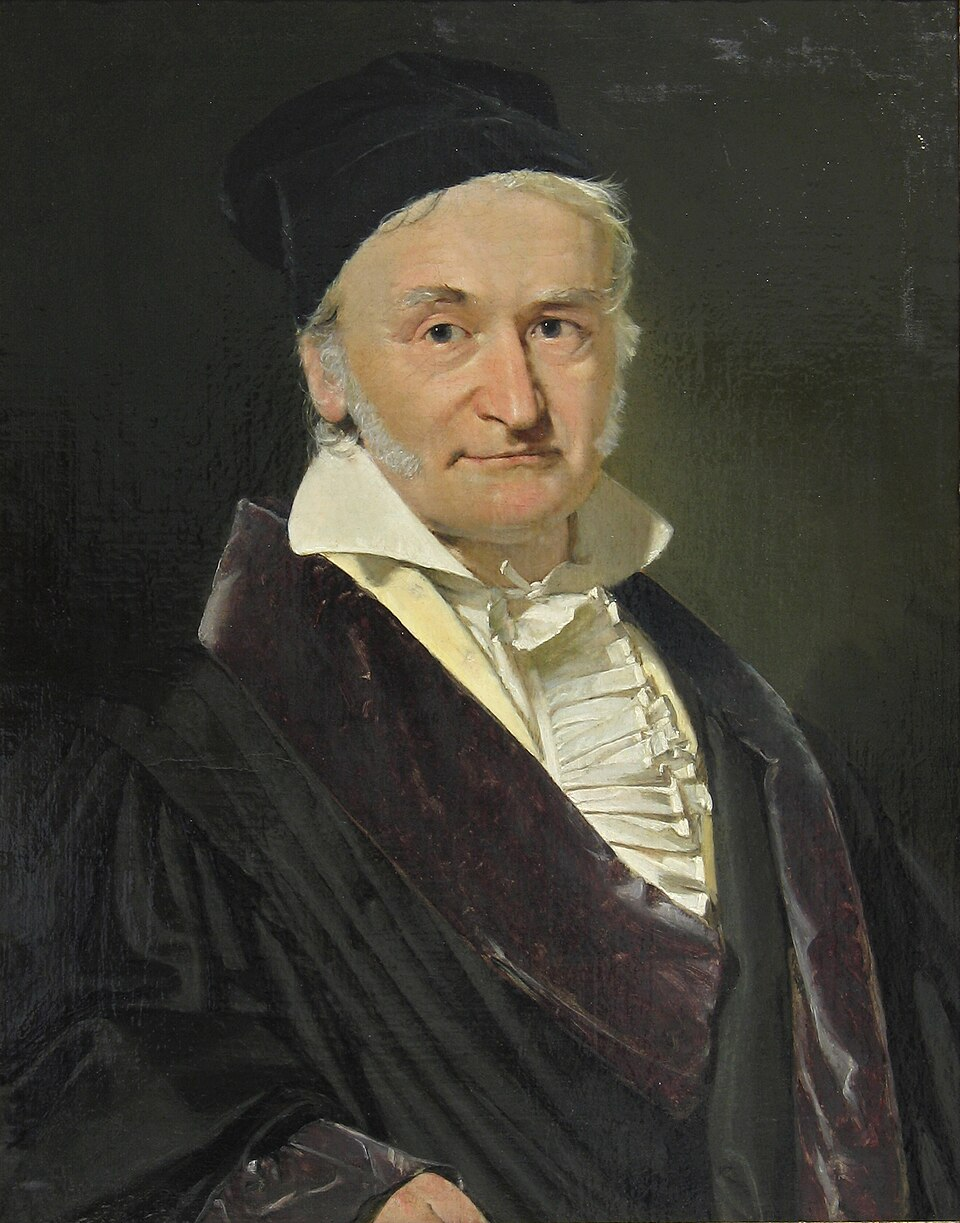
\includegraphics[height=0.56\textheight]{ch2_gauss_1840.jpg}\\[1mm]
\imgcap{Carl Friedrich Gauss (1777--1855)}
\imgcredit{https://commons.wikimedia.org/wiki/File:Carl_Friedrich_Gauss_1840_by_Jensen.jpg}{Portret: Christian Albrecht Jensen (1840); domeniu public; Wikimedia Commons}
\end{column}
\end{columns}
\end{frame}

\begin{frame}{Definiție}
\itemsize{\small}
\begin{itemize}
    \item $X \sim N(\mu, \sigma^2)$ are \textbf{PDF} (probability density function, densitatea de probabilitate)
    \begin{itemize}
        \item $f(x) = \dfrac{1}{\sigma\sqrt{2\pi}} \exp\Big(-\dfrac{(x - \mu)^2}{2\sigma^2}\Big)$, \quad $x \in \mathbb{R}$
        \item doi parametri: media $\mu$ (poziția) și varianța $\sigma^2$ (împrăștierea)
    \end{itemize}
    \item \textbf{Distribuția Normală standard}: $Z = (X - \mu)/\sigma \sim N(0, 1)$
    \begin{itemize}
        \item \textbf{CDF} (cumulative distribution function, funcția de repartiție) este $\Phi(z) = P(Z \le z)$, fără formă închisă; se calculează cu tabele sau cu software
    \end{itemize}
    \item Probabilitățile lui $X$ se obțin din $Z$: $P(X \le x) = \Phi\big((x - \mu)/\sigma\big)$
    \item Cuantila de ordin $\alpha$: $x_\alpha = \mu + \sigma z_\alpha$, cu $z_{0{,}01} = -2{,}33$, $z_{0{,}05} = -1{,}64$
\end{itemize}
\end{frame}

\begin{frame}{Proprietăți folosite în finanțe}
\itemsize{\small}
\begin{itemize}
    \item Simetrică în jurul lui $\mu$: media = mediana = modul
    \item Asimetria $0$ și aplatizarea $3$ (definite în secțiunea 5)
    \item \textbf{Închisă la adunare}: dacă $X \sim N(\mu_1, \sigma_1^2)$ și $Y \sim N(\mu_2, \sigma_2^2)$ sînt independente, atunci $X + Y \sim N(\mu_1 + \mu_2, \sigma_1^2 + \sigma_2^2)$
    \begin{itemize}
        \item randamentul logaritmic pe $h$ zile în modelul de referință: $r_t(h) \sim N(h\mu, h\sigma^2)$
        \item volatilitatea crește cu $\sqrt{h}$: regula rădăcinii pătrate a timpului din \sfmchlink{https://danpele.github.io/SFM/RO/Cursuri/capitol1_date_randamente_indicatori.pdf}{Capitolul 1}
    \end{itemize}
    \item Orice combinație liniară de randamente cu distribuție Normală multivariată este Normală: randamentele portofoliilor rămîn Normale
    \item Complet determinată de doi parametri: dacă știm $\mu$ și $\sigma$, putem calcula orice probabilitate
\end{itemize}
\end{frame}

\begin{frame}{Regula 68--95--99,7}
\itemsize{\footnotesize}
\begin{center}
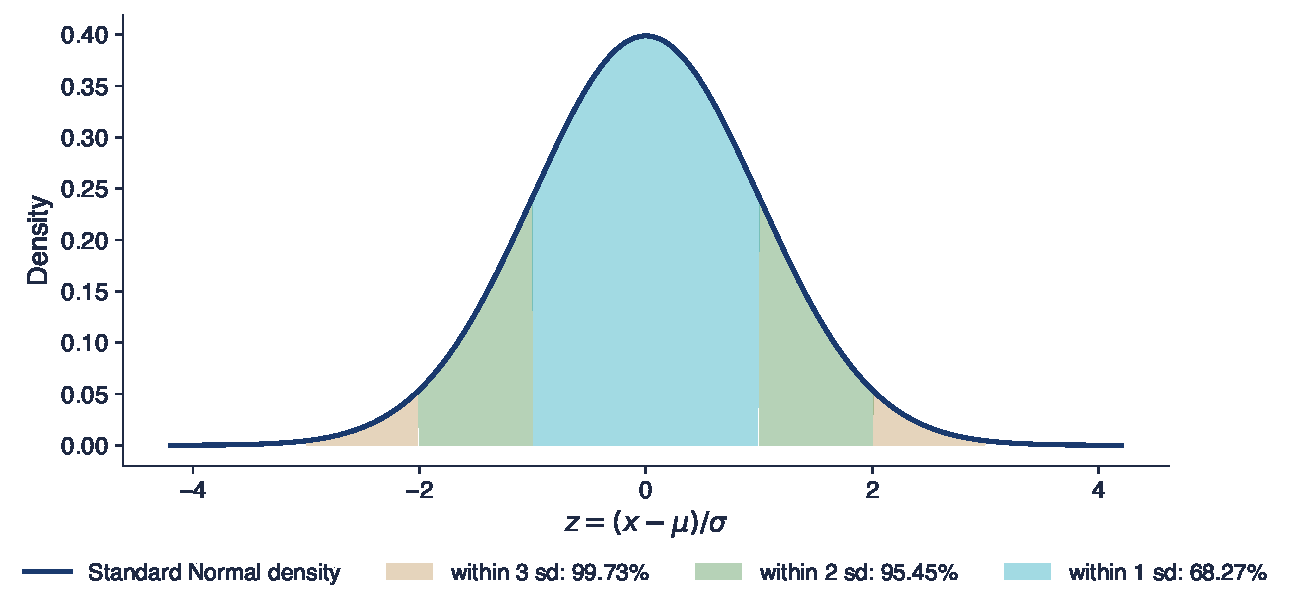
\includegraphics[width=0.97\textwidth,height=0.62\textheight,keepaspectratio]{sfm_ch2_normal_pdf.pdf}
\end{center}
\vspace{-0.25cm}
\begin{itemize}
    \item La cel mult 1, 2 și 3 abateri standard de medie: 68{,}27\%, 95{,}45\% și 99{,}73\% din probabilitate
    \item Dincolo de 3 abateri standard: o zi din 370; cozile distribuției Normale scad ca $e^{-z^2/2}$, foarte repede
\end{itemize}
\sfmquantlet{Ch_02}{SFM_ch2_normal_lognormal}
\end{frame}

\begin{frame}{Cît de rare sînt mișcările mari în cazul distribuției Normale?}
\itemsize{\small}
\begin{center}
\footnotesize
\begin{tabular}{crrr}
\toprule
$k$ & $P(|Z| > k)$ & o dată la \dots\ zile de tranzacționare & o dată la \dots\ ani \\
\midrule
1 & ${0{,}3173}$ & 3 & 0{,}013 \\
2 & ${0{,}0455}$ & 22 & 0{,}087 \\
3 & ${2{,}7 \times 10^{-3}}$ & 370 & 1{,}5 \\
4 & ${6{,}3 \times 10^{-5}}$ & 15\,787 & 63 \\
5 & ${5{,}7 \times 10^{-7}}$ & 1\,744\,278 & 6\,922 \\
6 & ${2{,}0 \times 10^{-9}}$ & 506\,797\,346 & 2\,011\,101 \\
\bottomrule
\end{tabular}
\end{center}
\begin{itemize}
    \item Anii sînt calculați cu 252 de zile de tranzacționare pe an
    \item Fiecare abatere standard în plus face o mișcare de 7 pînă la 291 de ori mai rară
    \item O zi de 6 sigma n-ar trebui să apară în toată istoria burselor
\end{itemize}\sfmquantlet{Ch_02}{SFM_ch2_normal_lognormal}
\end{frame}

\begin{frame}{Exemplu lucrat: pierderile mari ale S\&P 500}
\itemsize{\footnotesize}
\begin{itemize}
    \item S\&P 500, 2010--2026: $n = 4\,201$ randamente logaritmice zilnice, media $0{,}045\%$, abaterea standard $1{,}08\%$
    \item O pierdere mai mare de 3\%: $z = (-3 - 0{,}045)/1{,}08 = -2{,}81$
    \begin{itemize}
        \item distribuția Normală: $\Phi(-2{,}81) = 0{,}25\%$, deci numărul așteptat de zile este $10{,}5$
        \item numărul observat: 49 de zile
    \end{itemize}
    \item O pierdere mai mare de 5\%: $z = -4{,}65$
    \begin{itemize}
        \item distribuția Normală: $6{,}9 \times 10^{-3}$ zile așteptate; zile observate: 8
    \end{itemize}
    \item BET: 13 zile sub $-5\%$, față de $5{,}1 \times 10^{-3}$ așteptate
    \item Distribuția Normală subestimează frecvența pierderilor mari cu cîteva ordine de mărime
\end{itemize}
\end{frame}

\begin{frame}{Recapitulare: distribuția Normală}
\itemsize{\small}
\begin{itemize}
    \item Doi parametri, simetrică, închisă la adunare, volatilitatea crește cu $\sqrt{h}$
    \item Cozile ei sînt subțiri: o zi de 4 sigma o dată la 63 de ani
    \item Randamentele reale au mult mai multe mișcări mari decît permite ea
\end{itemize}
\end{frame}


%=============================================================================
\section{Distribuția lognormală}
%=============================================================================

\begin{frame}{De la randamente logaritmice Normale la prețuri lognormale}
\itemsize{\small}
\begin{itemize}
    \item O variabilă pozitivă $Y$ este \textbf{lognormală}, $Y \sim LN(m, s^2)$, dacă $\ln Y \sim N(m, s^2)$
    \item Densitatea: $f(y) = \dfrac{1}{y s\sqrt{2\pi}} \exp\Big(-\dfrac{(\ln y - m)^2}{2s^2}\Big)$, \quad $y > 0$
    \item În modelul de referință, $\ln(P_T/P_0) = r_1 + \dots + r_T \sim N(T\mu, T\sigma^2)$
    \begin{itemize}
        \item deci $P_T/P_0 \sim LN(T\mu, T\sigma^2)$ \refOsborne
    \end{itemize}
    \item De ce prețuri lognormale și nu Normale?
    \begin{itemize}
        \item prețurile nu pot fi negative; un preț cu distribuție Normală ar putea fi negativ
        \item randamentul simplu $R = e^r - 1 > -1$: nu puteți pierde mai mult decît ați investit
    \end{itemize}
    \item Manual: \refFHH, secț.~3.3; modelul Black--Scholes se bazează pe ea
\end{itemize}
\end{frame}

\begin{frame}{Media, mediana și modul}
\itemsize{\small}
\begin{itemize}
    \item Dacă $Y \sim LN(m, s^2)$:
    \item mediana $e^{m}$; modul $e^{m - s^2}$; media $E[Y] = e^{m + s^2/2}$
    \begin{itemize}
        \item întotdeauna modul $<$ mediana $<$ media: o coadă dreaptă lungă (asimetrie pozitivă)
    \end{itemize}
    \item Varianța: $\text{Var}(Y) = (e^{s^2} - 1)\,e^{2m + s^2}$
    \item Media rezultă din $E[e^X] = e^{m + s^2/2}$ pentru $X \sim N(m, s^2)$ (Seminarul 2 o deduce)
    \begin{itemize}
        \item termenul suplimentar $s^2/2$ este volatility drag din \sfmchlink{https://danpele.github.io/SFM/RO/Cursuri/capitol1_date_randamente_indicatori.pdf}{Capitolul 1}, privit din cealaltă direcție
    \end{itemize}
    \item Care dintre ele contează? Mediana este rezultatul unui investitor tipic; media este trasă în sus de cîteva traiectorii foarte bune
\end{itemize}
\end{frame}

\begin{frame}{Densități lognormale (SFElognormal)}
\itemsize{\footnotesize}
\begin{center}
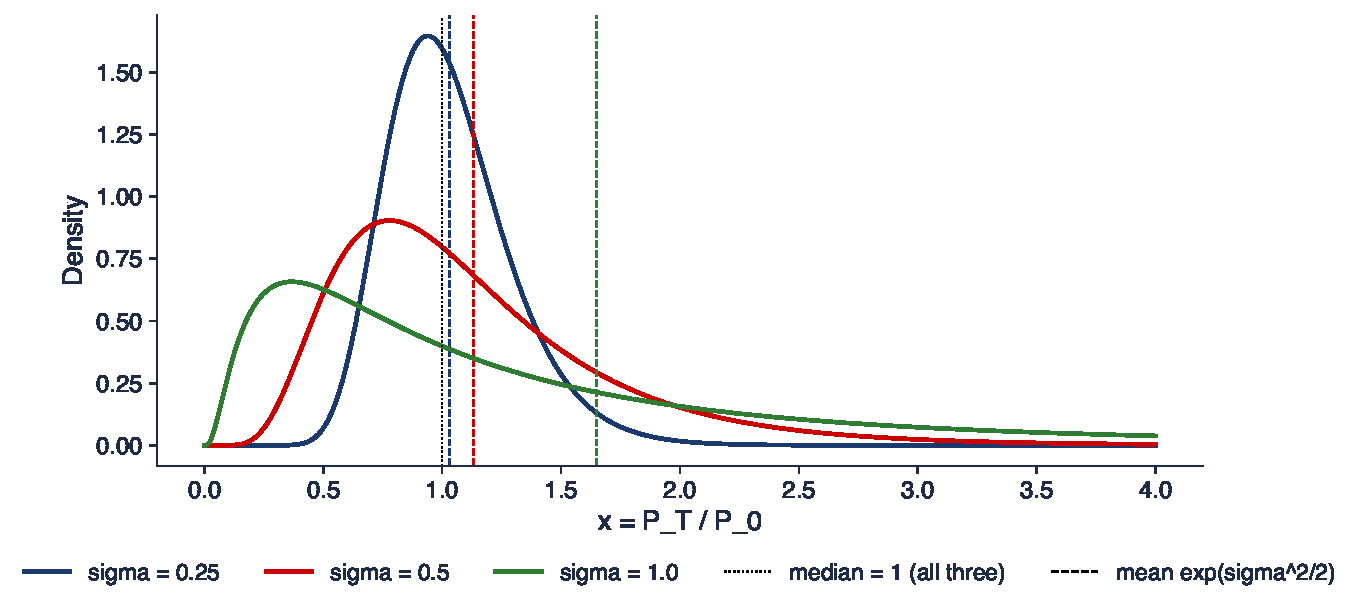
\includegraphics[width=0.97\textwidth,height=0.62\textheight,keepaspectratio]{sfm_ch2_lognormal.pdf}
\end{center}
\vspace{-0.25cm}
\begin{itemize}
    \item $m = 0$: mediana este 1 pentru toate cele trei curbe; liniile punctate marchează mediile
    \item $s = 0{,}25$: media $1{,}03$, modul $0{,}94$, aproape simetrică; $s = 1$: media $1{,}65$, modul $0{,}37$, asimetria $6{,}18$
    \item Orizonturi lungi sau volatilitate mare: distanța dintre medie și mediană crește
\end{itemize}
\sfmquantlet{Ch_02}{SFM_ch2_normal_lognormal}
\end{frame}

\begin{frame}{Exemplu lucrat: 100 de lei în BET}
\itemsize{\footnotesize}
\begin{itemize}
    \item BET, 2010--2026: randamentul logaritmic mediu anual $\mu = 11{,}6\%$ și volatilitatea $\sigma = 16{,}9\%$ (momentele zilnice $\times$ 251 și $\sqrt{251}$)
    \item După un an, $P_1/P_0 \sim LN(\mu, \sigma^2)$
    \begin{itemize}
        \item mediana $100e^{\mu} = 112{,}3$; media $100e^{\mu + \sigma^2/2} = 113{,}9$
        \item probabilitatea unei pierderi $\Phi(-\mu/\sigma) = 24{,}8\%$; cuantila de 5\% $100e^{\mu - 1{,}645\sigma} = 84{,}9$
    \end{itemize}
    \item După 10 ani, $P_{10}/P_0 \sim LN(10\mu, 10\sigma^2)$
    \begin{itemize}
        \item mediana 317{,}7; media 366{,}8; probabilitatea unei pierderi 1{,}5\%; cuantila de 5\% 131{,}6
    \end{itemize}
    \item Probabilitatea unei pierderi scade cu orizontul; după 10 ani, chiar și cuantila de 5\% depășește 100, dar numai dacă media istorică se menține
    \item Atenție: aceste rezultate moștenesc toate slăbiciunile modelului Normal al randamentelor logaritmice
\end{itemize}
\end{frame}

\begin{frame}{Recapitulare: distribuția lognormală}
\itemsize{\small}
\begin{itemize}
    \item Randamente logaritmice Normale $\Rightarrow$ prețuri lognormale: pozitive, asimetrice la dreapta
    \item Mediana $e^m$ sub media $e^{m + s^2/2}$: diferența este volatility drag
    \item Raportați mediana și o cuantilă joasă, nu doar media
\end{itemize}
\end{frame}


%=============================================================================
\section{Teorema limită centrală}
%=============================================================================

\begin{frame}{Tabla lui Galton}
\itemsize{\small}
\begin{columns}[T]
\begin{column}{0.52\textwidth}
\begin{itemize}
    \item Francis Galton (1889): bilele cad printre rînduri de cuie și sar la stînga sau la dreapta cu probabilitatea $1/2$
    \item Poziția finală a unei bile este o \textbf{sumă} de multe șocuri mici independente
    \item Grămezile formează o curbă clopot: probabilități binomiale apropiate de densitatea Normală
    \item Același argument a fost folosit pentru randamente: un randament zilnic este suma multor variații mici de preț din timpul zilei
\end{itemize}
\end{column}
\begin{column}{0.44\textwidth}
\centering
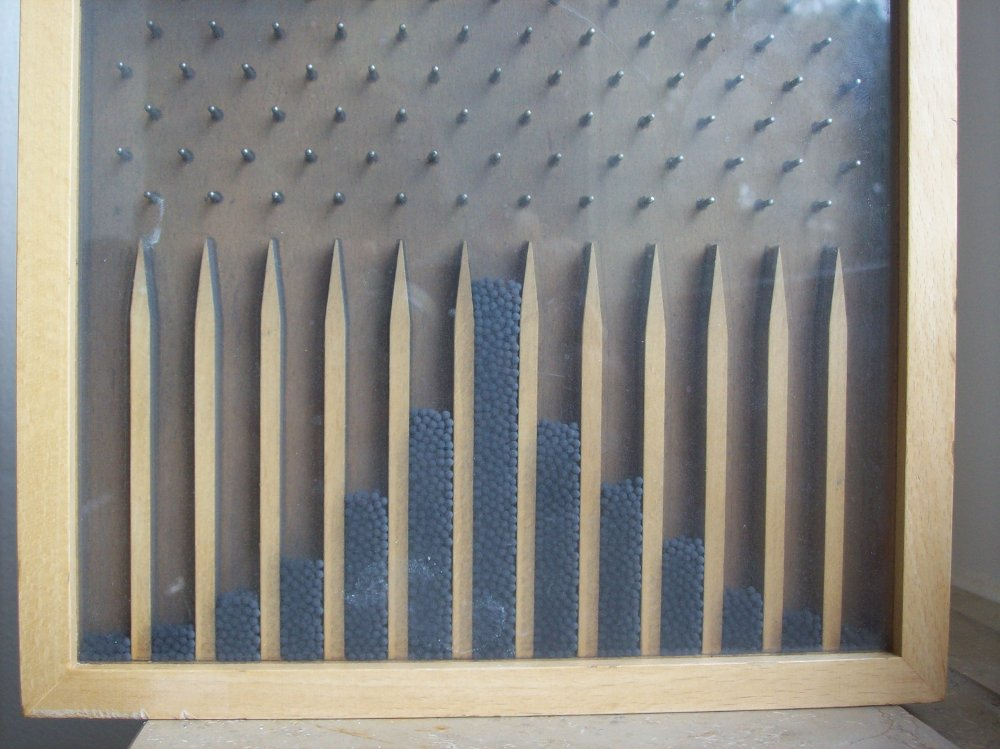
\includegraphics[height=0.45\textheight]{ch2_galton_board.jpg}\\[1mm]
\imgcap{O tablă Galton după căderea bilelor}
\imgcredit{https://commons.wikimedia.org/wiki/File:Galton_box_2.jpg}{Foto: Klaus-Dieter Keller (2010); domeniu public; Wikimedia Commons}
\end{column}
\end{columns}
\end{frame}

\begin{frame}{Teorema limită centrală}
\itemsize{\small}
\begin{itemize}
    \item \textbf{CLT} (Lindeberg--Lévy): $X_1, \dots, X_n$ i.i.d. cu media $\mu$ și varianța finită $\sigma^2$
    \begin{itemize}
        \item $\dfrac{\sqrt{n}\,(\bar X_n - \mu)}{\sigma} \xrightarrow{d} N(0, 1)$ cînd $n \to \infty$
        \item echivalent, suma $X_1 + \dots + X_n$ este aproximativ $N(n\mu, n\sigma^2)$
    \end{itemize}
    \item Trei condiții
    \begin{itemize}
        \item independență; distribuție identică; varianță finită
    \end{itemize}
    \item Cît de repede? Eroarea scade ca $1/\sqrt{n}$ și crește cu asimetria lui $X$ (marginea Berry--Esseen)
    \item Explică de ce distribuția Normală apare peste tot și de ce intervalele de încredere pentru medie se construiesc cu distribuția Normală
\end{itemize}
\end{frame}

\begin{frame}{CLT în practică (SFEclt)}
\itemsize{\footnotesize}
\begin{center}
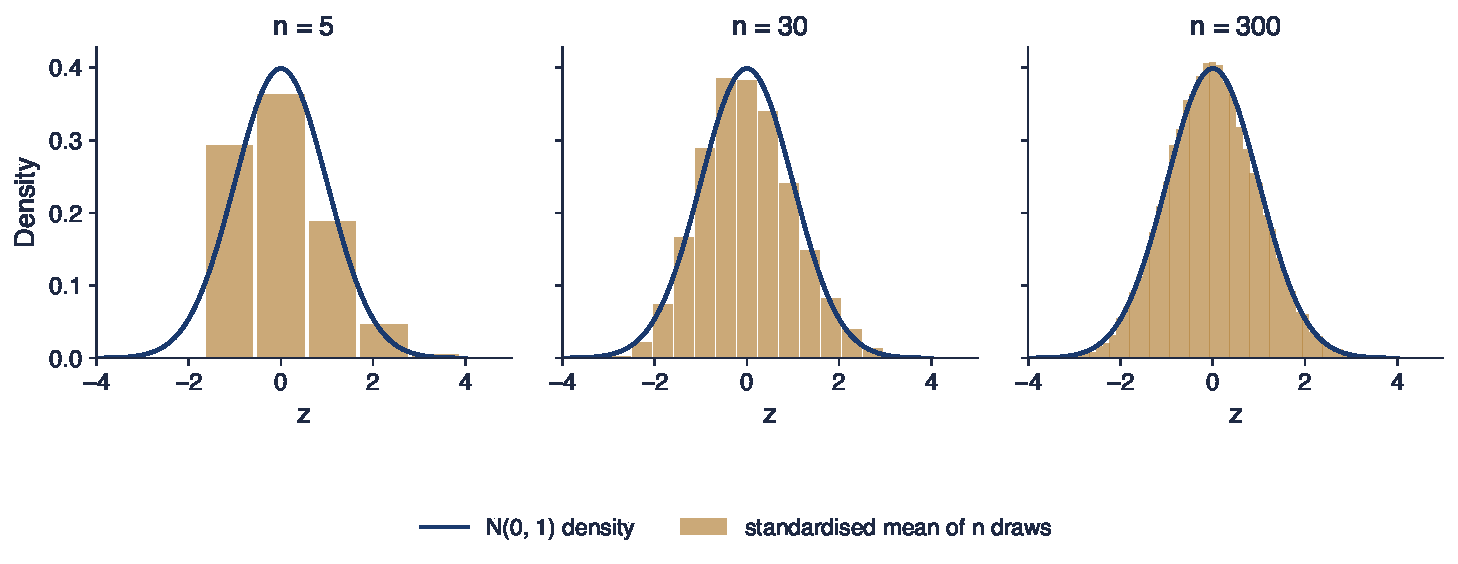
\includegraphics[width=0.97\textwidth,height=0.60\textheight,keepaspectratio]{sfm_ch2_clt.pdf}
\end{center}
\vspace{-0.25cm}
\begin{itemize}
    \item Media standardizată a $n$ extrageri Bernoulli($0{,}2$) (o variabilă asimetrică), 20\,000 de simulări
    \item Ponderea peste $1{,}96$: 5{,}8\% pentru $n = 5$, 2{,}7\% pentru $n = 30$, 2{,}8\% pentru $n = 300$; distribuția Normală: 2{,}5\%
    \item Asimetria mediei, $(1 - 2p)/\sqrt{np(1-p)}$: $0{,}67$, $0{,}27$, $0{,}09$
\end{itemize}
\sfmquantlet{Ch_02}{SFM_ch2_clt_normal_approx}
\end{frame}

\begin{frame}{Aproximarea Normală a distribuției binomiale (SFENormalApprox)}
\itemsize{\footnotesize}
\begin{center}
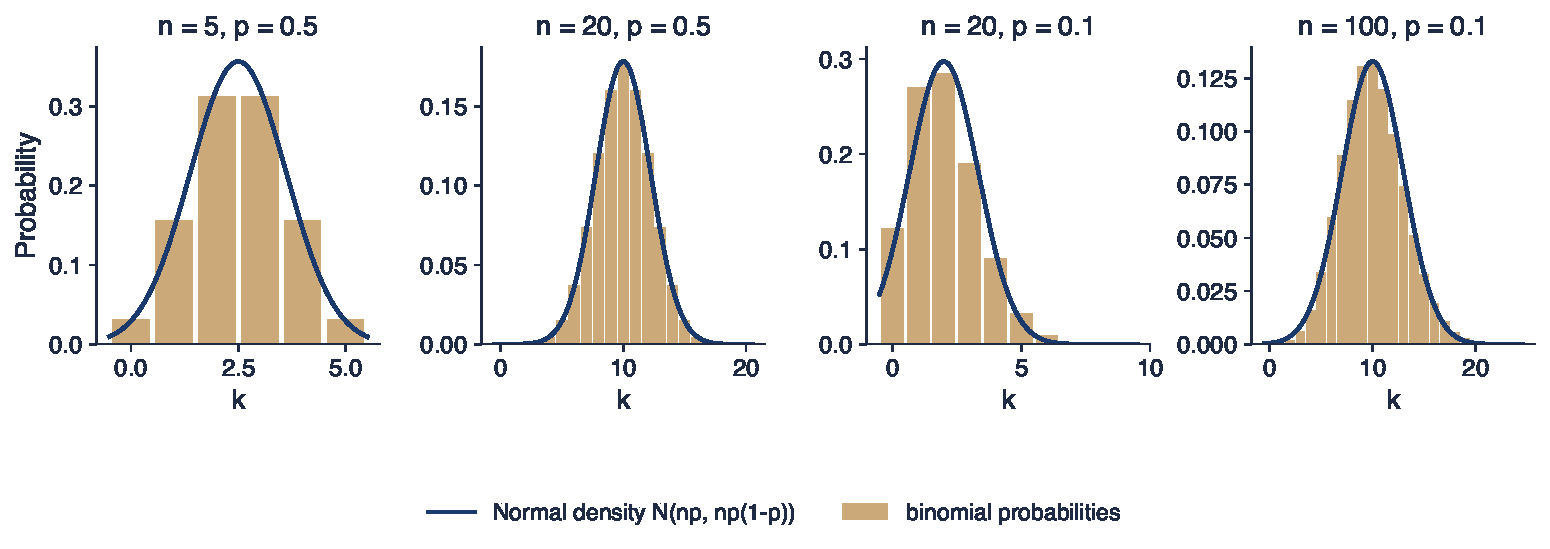
\includegraphics[width=0.97\textwidth,height=0.60\textheight,keepaspectratio]{sfm_ch2_normal_approx.pdf}
\end{center}
\vspace{-0.25cm}
\begin{itemize}
    \item $B(n, p) \approx N\big(np, np(1-p)\big)$; cu corecția de continuitate, $P(X \le k) \approx \Phi\big((k + 0{,}5 - np)/\sqrt{np(1-p)}\big)$
    \item Cea mai mare eroare a CDF: $0{,}001$ pentru $n = 20, p = 0{,}5$; $0{,}037$ pentru $n = 20, p = 0{,}1$; $0{,}017$ pentru $n = 100, p = 0{,}1$
    \item Regulă practică: aproximarea este bună cînd $np(1-p)$ este mare (cel puțin circa 9)
\end{itemize}
\sfmquantlet{Ch_02}{SFM_ch2_clt_normal_approx}
\end{frame}

\begin{frame}{Întrebare pentru sală: devin randamentele zilnice Normale datorită CLT?}
\itemsize{\small}
\begin{itemize}
    \item Un randament logaritmic zilnic este suma a mii de randamente logaritmice din timpul zilei
    \item \textbf{Ce credeți?} Ar trebui atunci randamentele zilnice să fie aproape Normale?
    \item \textbf{Răspuns}: nu neapărat; fiecare condiție a CLT poate fi încălcată
    \begin{itemize}
        \item dependență: zilele calme și cele agitate vin în grupuri (secțiunea 8)
        \item distribuție schimbătoare: volatilitatea diferă de la o zi la alta
        \item varianță infinită: \refMandelbrot{} a propus-o pentru prețurile bumbacului (\sfmchlink{https://danpele.github.io/SFM/RO/Cursuri/capitol3_distributii_alfa_stabile.pdf}{Capitolul 3}, distribuții $\alpha$-stabile)
    \end{itemize}
    \item Datele decid: secțiunile următoare măsoară cît de departe sînt randamentele de distribuția Normală
\end{itemize}
\end{frame}

\begin{frame}{Recapitulare: teorema limită centrală}
\itemsize{\small}
\begin{itemize}
    \item Sumele multor termeni i.i.d. cu varianță finită sînt aproximativ Normale
    \item Convergența este mai lentă pentru variabile asimetrice; $np(1-p) \ge 9$ pentru distribuția binomială
    \item Randamentele pot încălca independența, distribuția identică sau varianța finită
\end{itemize}
\end{frame}


%=============================================================================
\section{Momentele și forma unei distribuții}
%=============================================================================

\begin{frame}{Patru momente}
\itemsize{\small}
\begin{itemize}
    \item Media $\mu = E[X]$; varianța $\sigma^2 = E[(X - \mu)^2]$
    \item \textbf{Asimetria} (skewness): $\gamma_1 = E[(X - \mu)^3]/\sigma^3$
    \begin{itemize}
        \item $\gamma_1 < 0$: o coadă stîngă mai lungă, pierderile mari mai frecvente decît cîștigurile mari
    \end{itemize}
    \item \textbf{Aplatizarea} (kurtosis): $\gamma_2 = E[(X - \mu)^4]/\sigma^4$; distribuția Normală: $\gamma_2 = 3$
    \begin{itemize}
        \item \textbf{excesul de aplatizare} $\gamma_2 - 3$: pozitiv înseamnă cozi groase și un centru înalt și îngust (distribuție \textbf{leptocurtică})
    \end{itemize}
    \item Ambele sînt adimensionale: descriu forma, nu poziția sau scala
    \item Puterile a patra fac aplatizarea foarte sensibilă la cîteva zile extreme
\end{itemize}
\end{frame}

\begin{frame}{Asimetria și aplatizarea în grafice}
\itemsize{\footnotesize}
\begin{center}
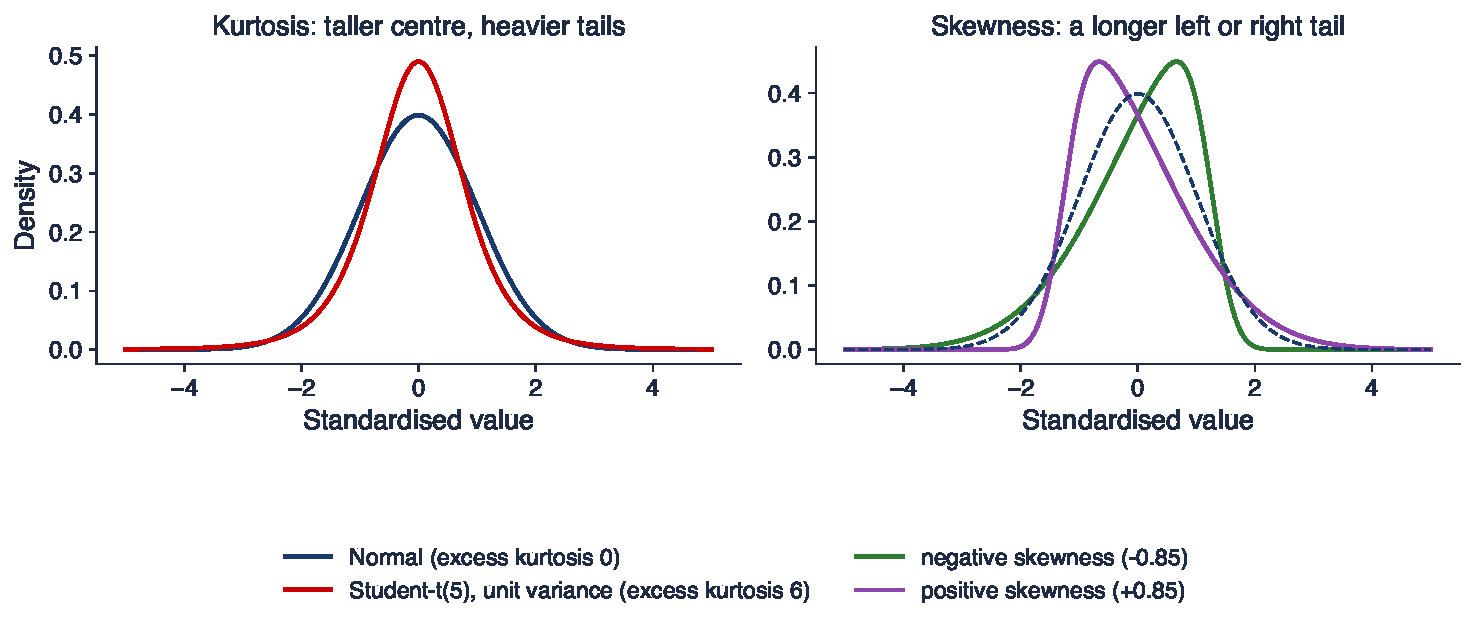
\includegraphics[width=0.97\textwidth,height=0.62\textheight,keepaspectratio]{sfm_ch2_shapes.pdf}
\end{center}
\vspace{-0.25cm}
\begin{itemize}
    \item Stînga: aceeași medie și varianță; curba Student-$t(5)$ (secțiunea 7) are exces de aplatizare 6: mai multă masă în centru și în cozi, mai puțină în umeri
    \item Dreapta: densități skew-Normal cu asimetria $\pm 0{,}85$; curba punctată este distribuția Normală
\end{itemize}
\sfmquantlet{Ch_02}{SFM_ch2_moments_jarque_bera}
\end{frame}

\begin{frame}{Momentele de selecție}
\itemsize{\small}
\begin{itemize}
    \item Momentele centrate de selecție: $m_k = \frac1n \sum_{t=1}^n (r_t - \bar r)^k$
    \item Asimetria de selecție $S = m_3/m_2^{3/2}$; excesul de aplatizare de selecție $K = m_4/m_2^2 - 3$
    \item Dacă datele sînt i.i.d. Normale: $S \approx N(0, 6/n)$ și $K \approx N(0, 24/n)$
    \begin{itemize}
        \item cu $n = 4\,201$: erorile standard $\sqrt{6/n} = 0{,}038$ și $\sqrt{24/n} = 0{,}076$
    \end{itemize}
    \item Aceste erori standard sînt valabile doar în ipoteza de normalitate; pentru date cu cozi groase sînt mult prea mici (Seminarul 2, B1)
    \item Exerciții din manual: \refFHHex
\end{itemize}
\end{frame}

\begin{frame}{Randamente logaritmice zilnice: momente, 2010--2026}
\itemsize{\footnotesize}
\begin{center}
\footnotesize
\begin{tabular}{lrrrrrrr}
\toprule
Seria & din & $n$ & Media \% & Ab. std. \% & Asim. & Exces apl. & Min \% \\
\midrule
S\&P 500 & 2010 & 4\,201 & $0{,}045$ & $1{,}08$ & $-0{,}61$ & $13{,}5$ & $-12{,}8$ \\
DAX & 2010 & 4\,244 & $0{,}034$ & $1{,}22$ & $-0{,}45$ & $7{,}4$ & $-13{,}1$ \\
BET & 2010 & 4\,186 & $0{,}046$ & $1{,}07$ & $-0{,}98$ & $17{,}9$ & $-11{,}9$ \\
Bitcoin & 2014 & 4\,384 & $0{,}118$ & $3{,}49$ & $-0{,}70$ & $12{,}0$ & $-46{,}5$ \\
OMV Petrom (SNP) & 2010 & 3\,815 & $0{,}076$ & $1{,}62$ & $-0{,}54$ & $8{,}9$ & $-15{,}8$ \\
BRD & 2010 & 3\,771 & $0{,}044$ & $1{,}66$ & $-0{,}38$ & $7{,}3$ & $-18{,}2$ \\
Nuclearelectrica (SNN) & 2013 & 2\,911 & $0{,}099$ & $1{,}52$ & $0{,}27$ & $5{,}1$ & $-9{,}4$ \\
Romgaz (SNG) & 2013 & 2\,909 & $0{,}090$ & $1{,}40$ & $-0{,}34$ & $5{,}3$ & $-11{,}0$ \\
\bottomrule
\end{tabular}
\end{center}
\begin{itemize}
    \item Toate seriile au exces de aplatizare între 5{,}1 (SNN) și 17{,}9 (BET): departe de 0
    \item Toate seriile, cu excepția SNN, au asimetrie negativă
    \item Cele mai proaste zile: S\&P 500 pe 16 martie 2020, BET pe 19 decembrie 2018 (OUG 114, taxa pe activele bancare), Bitcoin pe 12 martie 2020
\end{itemize}\sfmquantlet{Ch_02}{SFM_ch2_moments_jarque_bera}
\end{frame}

\begin{frame}{Randamentele DAX față de densitatea Normală (SFEDaxReturnDistribution)}
\itemsize{\footnotesize}
\begin{center}
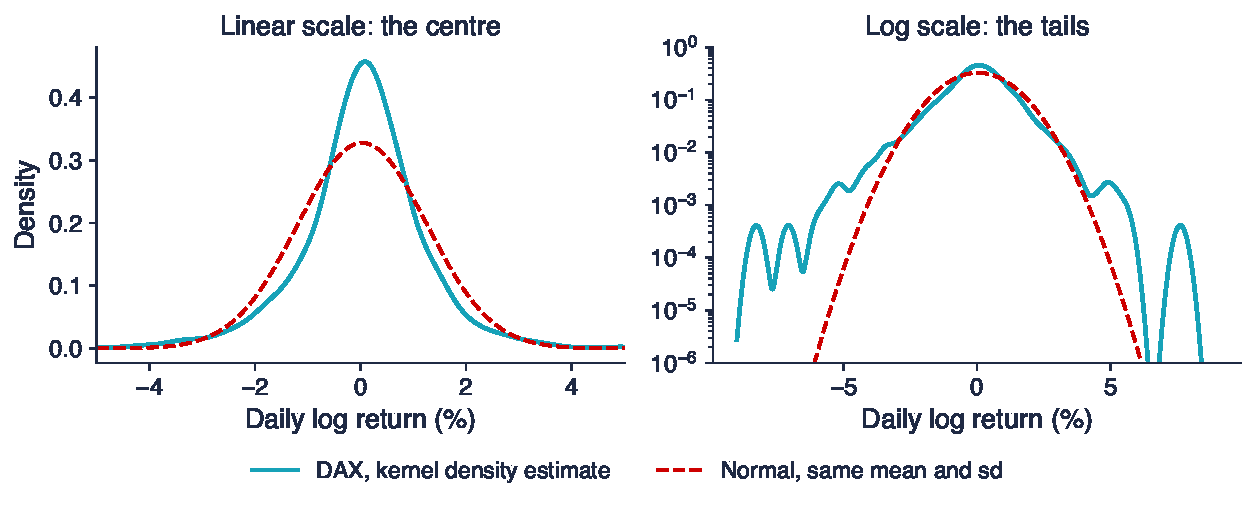
\includegraphics[width=0.97\textwidth,height=0.60\textheight,keepaspectratio]{sfm_ch2_dax_density.pdf}
\end{center}
\vspace{-0.25cm}
\begin{itemize}
    \item Estimatorul nucleu al densității (o histogramă netezită) față de densitatea Normală cu aceeași medie și abatere standard
    \item Centrul: vîrful densității 0{,}46 față de 0{,}33; 76{,}8\% din zile în interiorul unei abateri standard, față de 68{,}3\% pentru distribuția Normală
    \item Cozile (scară logaritmică): la $-6\%$ densitatea estimată este de 439 de ori mai mare decît densitatea Normală
\end{itemize}
\sfmquantlet{Ch_02}{SFM_ch2_moments_jarque_bera}
\end{frame}

\begin{frame}{Verificați datele înainte de a măsura cozile}
\itemsize{\footnotesize}
\begin{itemize}
    \item Banca Transilvania (TLV), 27--31 mai 2016: prețul de închidere scade de la 2{,}83 la 2{,}09 lei, data ex a unei distribuiri de acțiuni gratuite
    \item Prețul ajustat din datele noastre: 3{,}60, apoi 3{,}10, apoi 3{,}81
    \begin{itemize}
        \item randamente logaritmice $-15{,}0\%$ și $+20{,}5\%$ în două zile consecutive: ajustarea a fost aplicată cu o zi mai tîrziu
    \end{itemize}
    \item Excesul de aplatizare al TLV, 2010--2026: 17{,}5 cu aceste două zile, 13{,}5 fără ele
    \item Două zile greșite din mii schimbă aplatizarea cu o treime: de aceea TLV nu apare în tabelele acestui capitol
    \item Regula din \sfmchlink{https://danpele.github.io/SFM/RO/Cursuri/capitol1_date_randamente_indicatori.pdf}{Capitolul 1}: listați cele mai mari mișcări și verificați-le pe fiecare, mai ales perechile de salturi de semn opus
\end{itemize}
\end{frame}

\begin{frame}{Recapitulare: momente}
\itemsize{\small}
\begin{itemize}
    \item Asimetria măsoară lipsa simetriei, excesul de aplatizare măsoară greutatea cozilor față de distribuția Normală
    \item Randamentele zilnice: în general asimetrie negativă și exces de aplatizare între 5 și 18
    \item Aplatizarea este determinată de cîteva zile: verificați-le înainte de a avea încredere în ea
\end{itemize}
\end{frame}


%=============================================================================
\section{Testarea normalității: Jarque--Bera și QQ plots}
%=============================================================================

\begin{frame}{Testul Jarque--Bera}
\itemsize{\small}
\begin{itemize}
    \item $H_0$: datele sînt Normale, deci asimetria $= 0$ și excesul de aplatizare $= 0$
    \item Statistica \textbf{JB} \refJBa, \refJBb: $\text{JB} = \dfrac{n}{6}\Big(S^2 + \dfrac{K^2}{4}\Big)$
    \begin{itemize}
        \item suma a două statistici standardizate la pătrat: $(S/\sqrt{6/n})^2 + (K/\sqrt{24/n})^2$
    \end{itemize}
    \item În ipoteza $H_0$ și pentru $n$ mare: $\text{JB} \sim \chi^2(2)$; respingem la 5\% dacă $\text{JB} > 5{,}99$
    \item Este simplu, folosește doar două momente și este testul raportat de regulă în finanțele empirice
\end{itemize}
\end{frame}

\begin{frame}{Exemplu lucrat: Jarque--Bera pentru S\&P 500}
\itemsize{\small}
\begin{itemize}
    \item $n = 4\,201$, $S = -0{,}61$, $K = 13{,}5$
    \item $\text{JB} = 700{,}2 \times (0{,}367 + 45{,}5) = 32\,113$
    \item Valoarea critică 5{,}99: normalitatea este respinsă; valoarea $p$ este practic zero
    \item Termenul de aplatizare domină: aproape toată valoarea JB provine din $K^2/4$
    \item JB pentru celelalte serii: BET 56\,762, DAX 9\,909, Bitcoin 26\,482, SNN 3\,174
    \begin{itemize}
        \item toate respinse la orice nivel uzual
    \end{itemize}
\end{itemize}
\end{frame}

\begin{frame}{Limitele testului Jarque--Bera}
\itemsize{\small}
\begin{itemize}
    \item Cu mii de observații respinge chiar și abateri foarte mici
    \begin{itemize}
        \item raportați mărimea lui $S$ și $K$, nu doar valoarea $p$
    \end{itemize}
    \item Testul presupune date i.i.d.; cu volatility clustering, erorile standard ale lui $S$ și $K$ sînt prea mici
    \begin{itemize}
        \item S\&P 500: intervalul de 95\% pentru $K$ în ipoteza de normalitate: $[13{,}34; 13{,}64]$; intervalul bootstrap: $[6{,}7; 20{,}6]$ (Seminarul 2, B1)
    \end{itemize}
    \item Respingerea arată că datele nu sînt Normale, dar nu indică ce distribuție urmează
    \item Alte teste (Kolmogorov--Smirnov, Anderson--Darling) compară întreaga CDF: \sfmchlink{https://danpele.github.io/SFM/RO/Cursuri/capitol6_selectia_modelului_managementul_riscului.pdf}{Capitolul 6}
\end{itemize}
\end{frame}

\begin{frame}{QQ plots}
\itemsize{\small}
\begin{itemize}
    \item Un \textbf{QQ plot} (quantile--quantile plot, graficul cuantilă--cuantilă) compară cuantilele empirice cu cele ale unui model \refWG
    \begin{itemize}
        \item ordonați datele: $r_{(1)} \le r_{(2)} \le \dots \le r_{(n)}$
        \item reprezentați $r_{(i)}$ în funcție de cuantila modelului $F^{-1}\big((i - 0{,}5)/n\big)$
    \end{itemize}
    \item Cum se citește
    \begin{itemize}
        \item puncte pe prima bisectoare: modelul se potrivește
        \item o formă de S, capătul de jos sub dreaptă și cel de sus deasupra: cozi mai groase decît ale modelului
        \item un singur capăt se îndepărtează de dreaptă: asimetrie
    \end{itemize}
    \item Spre deosebire de JB, arată \textbf{unde} greșește modelul: în centru, în umeri sau în cozi
\end{itemize}
\end{frame}

\begin{frame}{QQ plots față de distribuția Normală}
\itemsize{\footnotesize}
\begin{center}
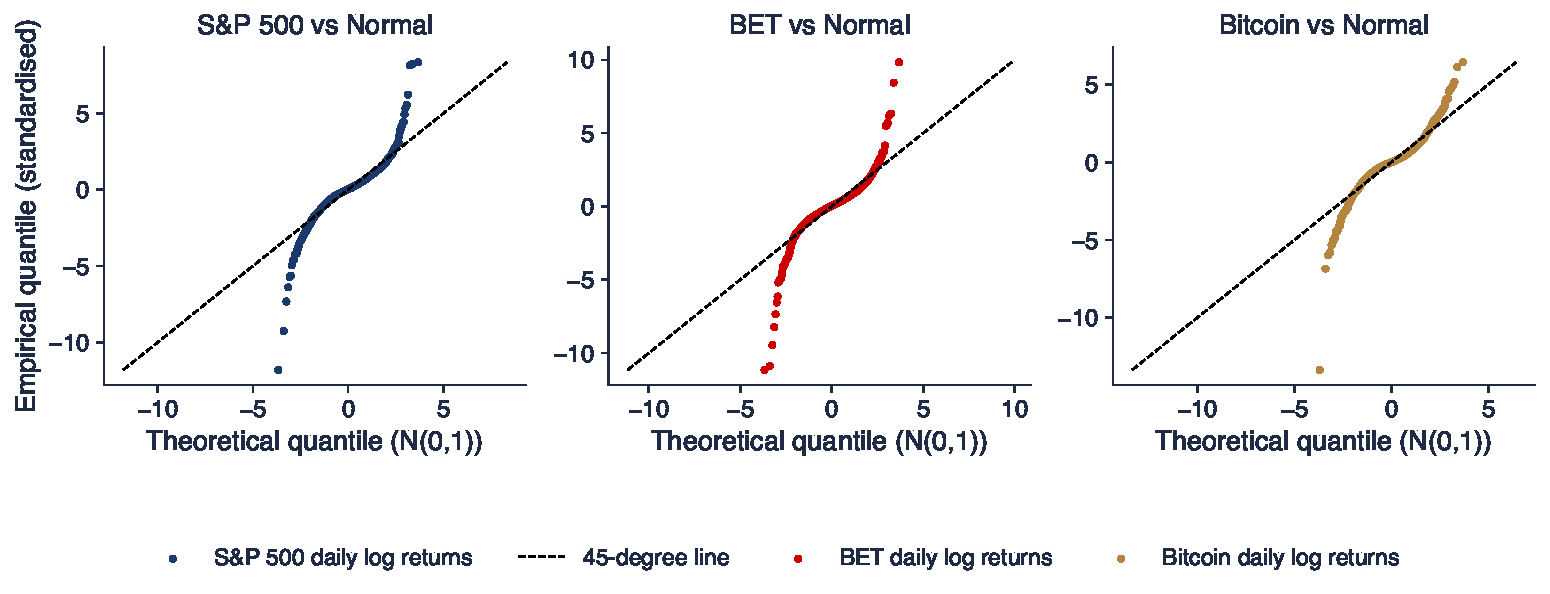
\includegraphics[width=0.97\textwidth,height=0.62\textheight,keepaspectratio]{sfm_ch2_qq_normal.pdf}
\end{center}
\vspace{-0.25cm}
\begin{itemize}
    \item Randamente standardizate față de cuantilele $N(0,1)$: toate trei se depărtează de dreaptă la ambele capete
    \item S\&P 500: cel mai mic randament standardizat $-11{,}8$, unde cuantila Normală este $-3{,}7$; BET: $-11{,}2$ față de $-3{,}7$
    \item Coada de jos se curbează mai mult decît cea de sus: asimetrie negativă
\end{itemize}
\sfmquantlet{Ch_02}{SFM_ch2_qq_plots}
\end{frame}

\begin{frame}{Recapitulare: testarea normalității}
\itemsize{\small}
\begin{itemize}
    \item JB combină asimetria și aplatizarea; respinge normalitatea pentru toate seriile
    \item Raportați mărimea abaterii; erorile standard din teoria Normală sînt prea mici
    \item QQ plots arată unde greșește modelul: aici, în ambele cozi
\end{itemize}
\end{frame}


%=============================================================================
\section{Distribuția Student-$t$}
%=============================================================================

\begin{frame}{„Student”: William Sealy Gosset}
\itemsize{\small}
\begin{columns}[T]
\begin{column}{0.58\textwidth}
\begin{itemize}
    \item Chimist și berar la Guinness, Dublin, lucra cu eșantioane mici de orz și hamei
    \item Fabrica de bere nu își lăsa angajații să publice sub propriul nume: a semnat „Student” \refStudent
    \item A dedus distribuția lui $(\bar X - \mu)/(s/\sqrt n)$ pentru date Normale: distribuția $t$
    \item În finanțe este folosită din alt motiv: cozile ei sînt mai groase decît cele ale distribuției Normale \refPraetz, \refBG
\end{itemize}
\end{column}
\begin{column}{0.38\textwidth}
\centering
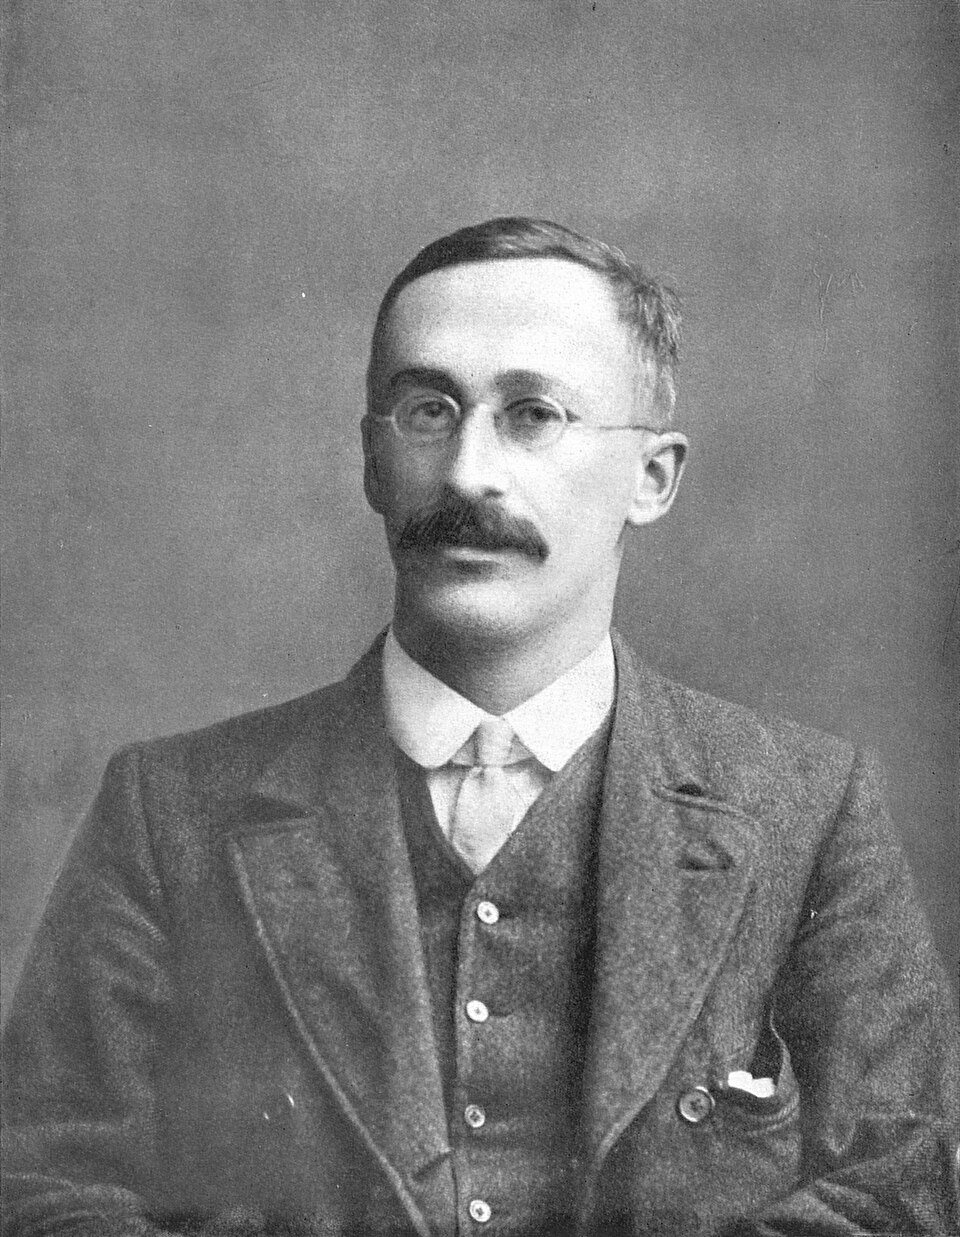
\includegraphics[height=0.56\textheight]{ch2_gosset_1908.jpg}\\[1mm]
\imgcap{William Sealy Gosset (1876--1937)}
\imgcredit{https://commons.wikimedia.org/wiki/File:William_Sealy_Gosset.jpg}{Foto: autor necunoscut (1908); domeniu public; Wikimedia Commons}
\end{column}
\end{columns}
\end{frame}

\begin{frame}{Definiție}
\itemsize{\small}
\begin{itemize}
    \item $T = Z/\sqrt{V/\nu}$, cu $Z \sim N(0,1)$ independentă de $V \sim \chi^2(\nu)$: $T \sim t(\nu)$
    \begin{itemize}
        \item $\nu > 0$: \textbf{gradele de libertate}, care controlează cozile
    \end{itemize}
    \item Densitatea: $f(x) = \dfrac{\Gamma\big((\nu+1)/2\big)}{\sqrt{\nu\pi}\,\Gamma(\nu/2)} \Big(1 + \dfrac{x^2}{\nu}\Big)^{-(\nu+1)/2}$
    \item Versiunea cu parametri de poziție și de scală pentru randamente: $r = m + s\,T$, cu poziția $m$, scala $s$ și $\nu$
    \item Cînd $\nu \to \infty$, $t(\nu) \to N(0,1)$: distribuția Normală este un caz limită
\end{itemize}
\end{frame}

\begin{frame}{Momente și cozi}
\itemsize{\small}
\begin{itemize}
    \item Media $0$ dacă $\nu > 1$; varianța $\nu/(\nu - 2)$ dacă $\nu > 2$; excesul de aplatizare $6/(\nu - 4)$ dacă $\nu > 4$
    \item Momentele de ordin $\nu$ și mai mare sînt infinite
    \begin{itemize}
        \item $\nu \le 4$: aplatizare infinită; $\nu \le 2$: varianță infinită
    \end{itemize}
    \item \textbf{Cozi de tip putere}: $P(|T| > x) \approx c\,x^{-\nu}$ pentru $x$ mare
    \begin{itemize}
        \item coada Normală scade ca $e^{-x^2/2}$, mult mai repede decît orice putere
        \item $\nu$ este și \textbf{indicele de coadă}, estimat direct în \sfmchlink{https://danpele.github.io/SFM/RO/Cursuri/capitol5_cozi_groase_evt.pdf}{Capitolul 5}
    \end{itemize}
    \item Pentru comparația cu distribuția Normală la aceeași varianță, folosiți $T\sqrt{(\nu - 2)/\nu}$, care are varianța 1
\end{itemize}
\end{frame}

\begin{frame}{Densități Student-$t$ cu varianța 1}
\itemsize{\footnotesize}
\begin{center}
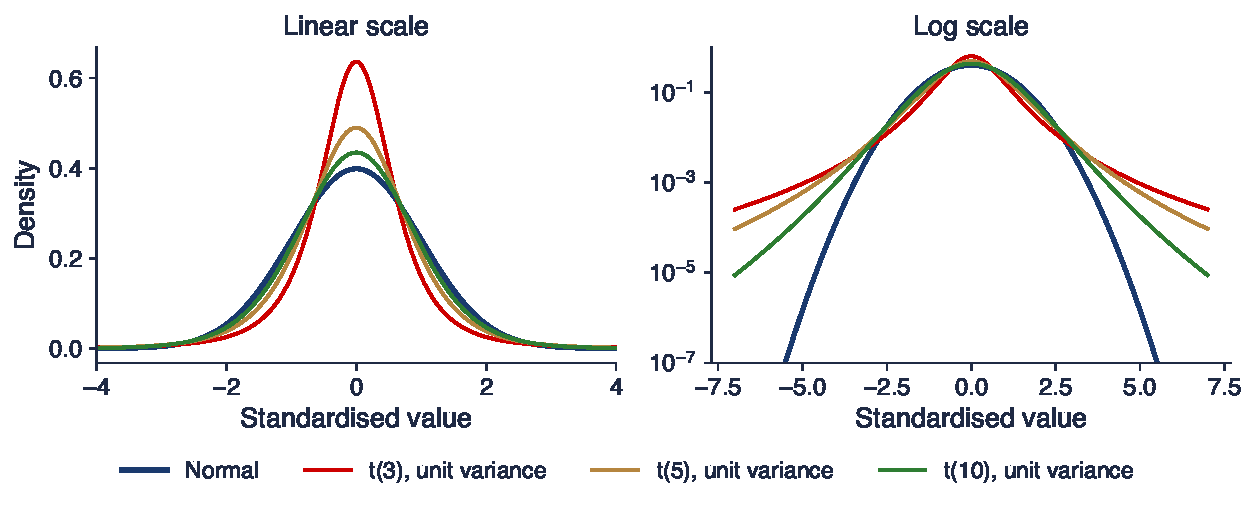
\includegraphics[width=0.97\textwidth,height=0.60\textheight,keepaspectratio]{sfm_ch2_t_densities.pdf}
\end{center}
\vspace{-0.25cm}
\begin{itemize}
    \item $\nu$ mai mic: centru mai înalt și cozi mai groase; pe scara logaritmică, cozile Normale scad ca o parabolă
    \item $P(|X| > 4)$ la varianța 1: $t(3)$ 0{,}62\%, $t(5)$ 0{,}36\%, $t(10)$ 0{,}12\%, distribuția Normală 0{,}0063\%
    \item Cu $\nu = 5$, o zi de 4 sigma este de 56 de ori mai probabilă decît în cazul distribuției Normale
\end{itemize}
\sfmquantlet{Ch_02}{SFM_ch2_student_t_fit}
\end{frame}

\begin{frame}{Estimarea unei distribuții Student-$t$ prin verosimilitate maximă}
\itemsize{\small}
\begin{itemize}
    \item \textbf{MLE} (maximum likelihood estimation, estimarea prin verosimilitate maximă): alegem $(\nu, m, s)$ care maximizează log-verosimilitatea
    \begin{itemize}
        \item $\ell(\nu, m, s) = \sum_{t=1}^n \ln f\big((r_t - m)/s; \nu\big) - n \ln s$
        \item fără formă închisă: un optimizator numeric (\texttt{scipy.stats.t.fit} în notebook)
    \end{itemize}
    \item \textbf{AIC} (Akaike information criterion, criteriul informațional Akaike) \refAkaike: $\text{AIC} = 2k - 2\ell$
    \begin{itemize}
        \item $k$ = numărul de parametri (2 pentru distribuția Normală, 3 pentru $t$); se preferă modelul cu AIC mai mic
        \item $\Delta\text{AIC} = \text{AIC}_{\text{Normal}} - \text{AIC}_{t} > 0$ favorizează $t$
    \end{itemize}
    \item Primele rezultate empirice pentru prețurile acțiunilor: \refPraetz, \refBG
\end{itemize}
\end{frame}

\begin{frame}{Distribuția Student-$t$ estimată: gradele de libertate, 2010--2026}
\itemsize{\footnotesize}
\begin{columns}[T]
\begin{column}{0.55\textwidth}
\begin{center}
\footnotesize
\begin{tabular}{lrrr}
\toprule
Seria & $\hat\nu$ & JB & $\Delta$AIC \\
\midrule
S\&P 500 & $2{,}78$ & 32\,113 & $1213$ \\
DAX & $3{,}31$ & 9\,909 & $739$ \\
BET & $2{,}96$ & 56\,762 & $1454$ \\
Bitcoin & $2{,}23$ & 26\,482 & $1335$ \\
OMV Petrom (SNP) & $3{,}79$ & 12\,832 & $679$ \\
BRD & $4{,}67$ & 8\,370 & $478$ \\
Nuclearelectrica (SNN) & $3{,}08$ & 3\,174 & $541$ \\
Romgaz (SNG) & $3{,}40$ & 3\,415 & $482$ \\
\bottomrule
\end{tabular}
\end{center}

\end{column}
\begin{column}{0.41\textwidth}
\begin{itemize}
    \item Toate valorile $\hat\nu$ între 2{,}23 (Bitcoin) și 4{,}67 (BRD)
    \item $\hat\nu < 4$ pentru 7 din cele 8 serii: modelul estimat are aplatizare infinită
    \item $\Delta$AIC este cel puțin 478: distribuția $t$ este preferată distribuției Normale pentru toate seriile
\end{itemize}
\end{column}
\end{columns}\sfmquantlet{Ch_02}{SFM_ch2_student_t_fit}
\end{frame}

\begin{frame}{S\&P 500: distribuția Normală și distribuția Student-$t$ estimate}
\itemsize{\footnotesize}
\begin{center}
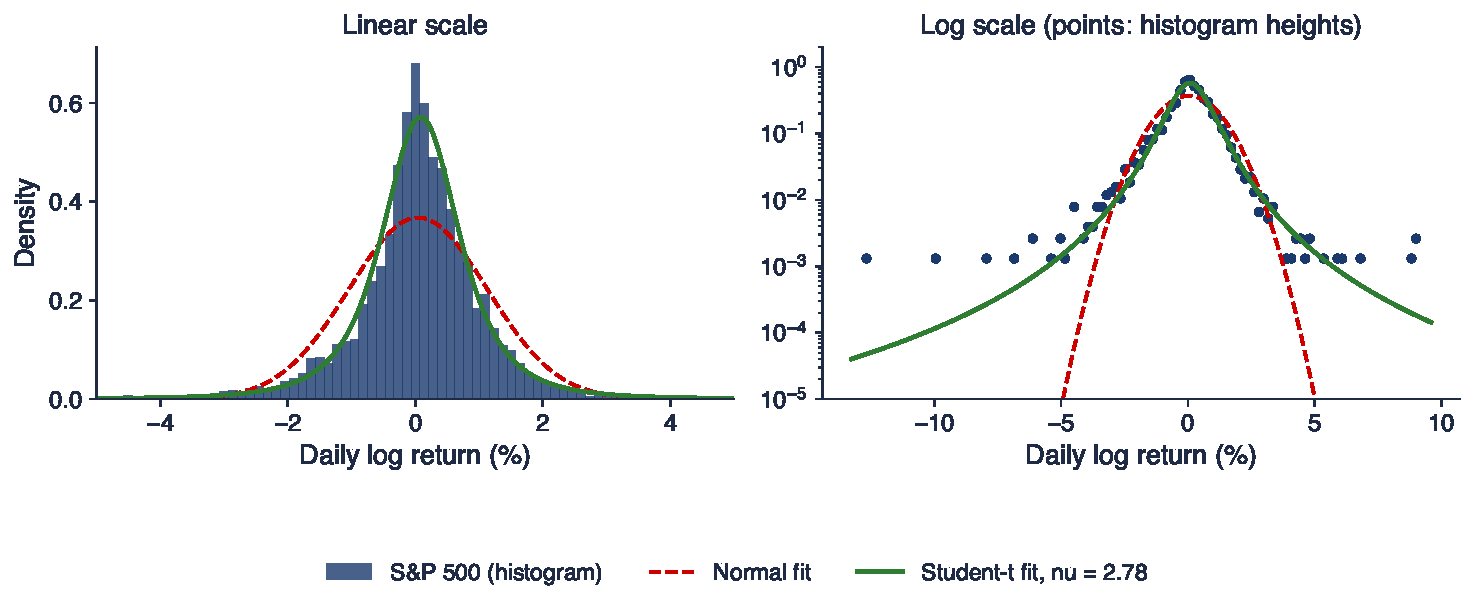
\includegraphics[width=0.97\textwidth,height=0.62\textheight,keepaspectratio]{sfm_ch2_t_fit_sp500.pdf}
\end{center}
\vspace{-0.25cm}
\begin{itemize}
    \item Scara liniară: distribuția $t$ ($\hat\nu = 2{,}78$) reproduce centrul înalt, pe care distribuția Normală nu îl reproduce
    \item Scara logaritmică: densitatea Normală scade abrupt dincolo de $\pm 4\%$; distribuția $t$ urmează cozile observate
\end{itemize}
\sfmquantlet{Ch_02}{SFM_ch2_student_t_fit}
\end{frame}

\begin{frame}{QQ plots față de distribuția Student-$t$ estimată}
\itemsize{\footnotesize}
\begin{center}
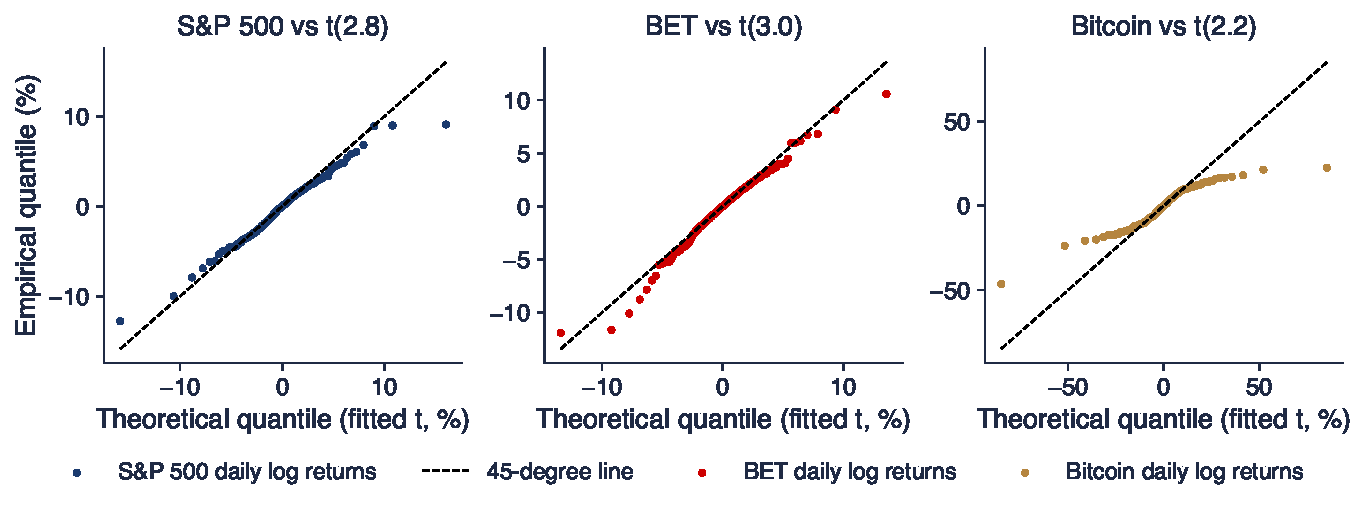
\includegraphics[width=0.97\textwidth,height=0.60\textheight,keepaspectratio]{sfm_ch2_qq_t.pdf}
\end{center}
\vspace{-0.25cm}
\begin{itemize}
    \item Centrul și cozile moderate se află acum pe dreaptă
    \item Extremele: distribuția $t$ estimată prevede minime mai mici decît cele observate: S\&P 500 $-15{,}8\%$ față de $-12{,}8\%$; Bitcoin $-85{,}0\%$ față de $-46{,}5\%$
    \item Cu $\hat\nu$ apropiat de 2, modelul supraestimează cuantilele cele mai extreme
\end{itemize}
\sfmquantlet{Ch_02}{SFM_ch2_qq_plots}
\end{frame}

\begin{frame}{Limitele distribuției Student-$t$}
\itemsize{\small}
\begin{itemize}
    \item \textbf{Simetria}: $t$ nu poate reproduce asimetria negativă
    \begin{itemize}
        \item există distribuții $t$ asimetrice, dar depășesc cadrul acestui capitol
    \end{itemize}
    \item \textbf{Independența}: un model $t$ i.i.d. nu are volatility clustering
    \begin{itemize}
        \item modelele GARCH cu erori $t$ le combină pe amîndouă \refBollerslev{} (Capitolul 9)
    \end{itemize}
    \item \textbf{Un singur indice de coadă}: un singur $\nu$ pentru ambele cozi și pentru centru
    \begin{itemize}
        \item teoria valorilor extreme modelează fiecare coadă separat (\sfmchlink{https://danpele.github.io/SFM/RO/Cursuri/capitol5_cozi_groase_evt.pdf}{Capitolul 5})
    \end{itemize}
    \item Rămîne cel mai simplu model cu cozi groase și o îmbunătățire mare față de distribuția Normală
\end{itemize}
\end{frame}

\begin{frame}{Recapitulare: Student-$t$}
\itemsize{\small}
\begin{itemize}
    \item Un parametru în plus, $\nu$, controlează cozile; cozi de tip putere, distribuția Normală cînd $\nu \to \infty$
    \item $\hat\nu$ estimat între 2 și 5 pentru randamentele zilnice; AIC preferă clar $t$
    \item Nu surprinde asimetria și volatility clustering
\end{itemize}
\end{frame}


%=============================================================================
\section{Faptele stilizate ale randamentelor}
%=============================================================================

\begin{frame}{Ce este un fapt stilizat?}
\itemsize{\small}
\begin{columns}[T]
\begin{column}{0.60\textwidth}
\begin{itemize}
    \item Un \textbf{fapt stilizat}: o proprietate statistică comună multor active, piețe și perioade \refCont
    \item Calitativ, nu exact: „cozi groase”, nu „$\nu = 3{,}2$”
    \item Rama Cont enumeră unsprezece; noi verificăm șase pe datele noastre
    \item Un model bun al randamentelor trebuie să le reproducă; modelul de referință i.i.d. Normal nu reproduce majoritatea lor
    \item Primele rezultate empirice: \refMandelbrot, \refFama
\end{itemize}
\end{column}
\begin{column}{0.36\textwidth}
\centering
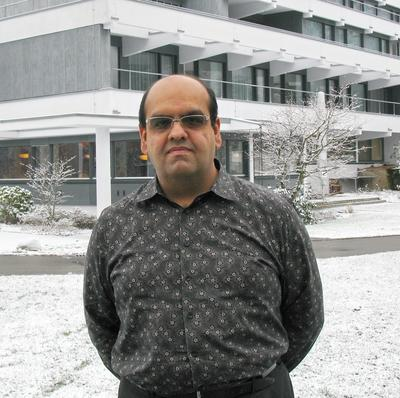
\includegraphics[height=0.42\textheight]{ch2_cont_2012.jpg}\\[1mm]
\imgcap{Rama Cont}
\imgcredit{https://commons.wikimedia.org/wiki/File:Rama_Cont_Oberwolfach_2012.jpg}{Foto: Renate Schmid (2012); CC BY-SA 2.0 DE; Wikimedia Commons}
\end{column}
\end{columns}
\end{frame}

\begin{frame}{Șase fapte stilizate}
\itemsize{\small}
\begin{itemize}
    \item \textbf{1. Cozi groase}: mișcările mari sînt mult mai frecvente decît prevede distribuția Normală
    \item \textbf{2. Gaussianitate agregată} (aggregational Gaussianity): randamentele pe orizonturi mai lungi sînt mai apropiate de distribuția Normală
    \item \textbf{3. Absența autocorelației liniare}: randamentele trecute aproape nu au putere de predicție pentru cele viitoare
    \item \textbf{4. Volatility clustering}: mișcările mari urmează mișcărilor mari, de orice semn
    \item \textbf{5. Efectul de levier} (leverage effect): scăderile cresc volatilitatea viitoare mai mult decît creșterile
    \item \textbf{6. Asimetria cîștig/pierdere}: pierderile mari sînt mai mari și mai frecvente decît cîștigurile mari
\end{itemize}
\end{frame}

\begin{frame}{Faptul 1: cozile groase în cifre}
\itemsize{\footnotesize}
\begin{center}
\footnotesize
\begin{tabular}{lrrrrrr}
\toprule
Seria & $n$ & $>3\sigma$ & $>4\sigma$ & $>5\sigma$ & $>6\sigma$ & $p$ (Poisson, $4\sigma$) \\
\midrule
S\&P 500 & 4\,201 & 62 & 28 & 12 & 8 & ${2 \times 10^{-46}}$ \\
DAX & 4\,244 & 56 & 20 & 5 & 4 & ${1 \times 10^{-30}}$ \\
BET & 4\,186 & 70 & 28 & 16 & 11 & ${2 \times 10^{-46}}$ \\
Bitcoin & 4\,384 & 80 & 29 & 10 & 4 & ${6 \times 10^{-48}}$ \\
Distribuția Normală, $n = 4\,201$ & & $11{,}34$ & $0{,}27$ & $2{,}4 \times 10^{-3}$ & $8{,}3 \times 10^{-6}$ &  \\
\bottomrule
\end{tabular}
\end{center}
\begin{itemize}
    \item $>k\sigma$: numărul zilelor cu $|r_t - \bar r| > k\,s$; ultimul rînd: numărul așteptat conform distribuției Normale
    \item $p$: probabilitatea de a observa cel puțin atîtea zile de 4 sigma, dacă numărul lor urmează distribuția Poisson cu media $n \times 6{,}3 \times 10^{-5}$ (ipoteza de normalitate)
    \item S\&P 500: de 105 de ori mai multe zile de 4 sigma decît permite distribuția Normală
\end{itemize}\sfmquantlet{Ch_02}{SFM_ch2_sigma_days}
\end{frame}

\begin{frame}{Faptul 1: zile de 4 sigma pe toate piețele}
\itemsize{\footnotesize}
\begin{center}
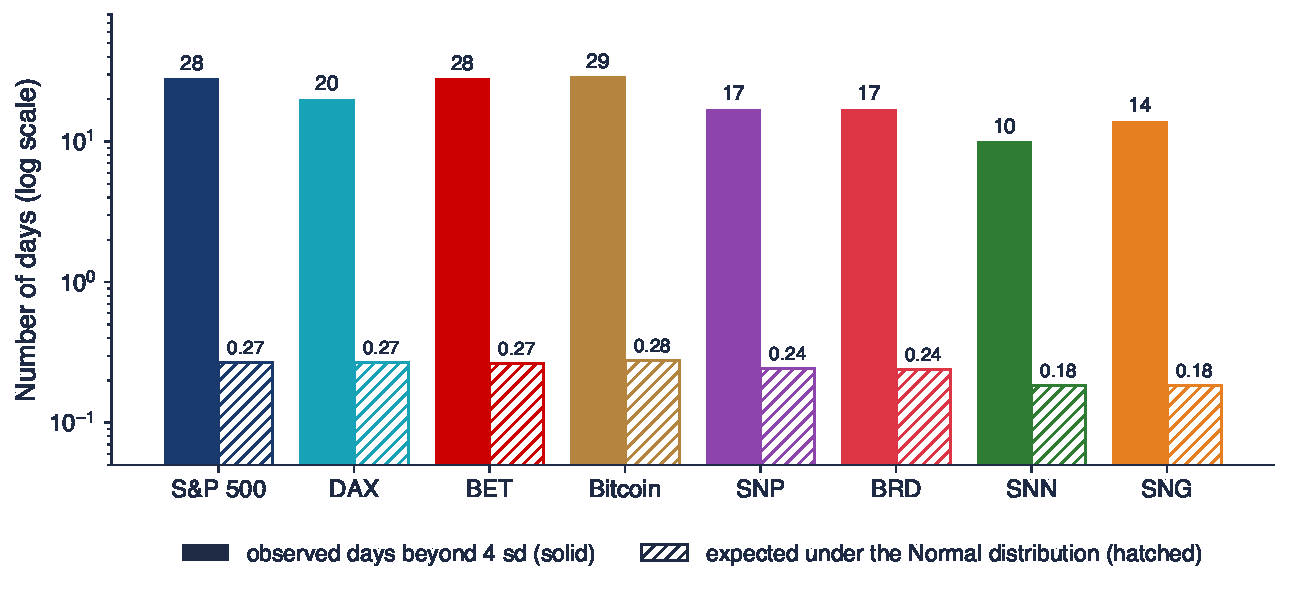
\includegraphics[width=0.97\textwidth,height=0.60\textheight,keepaspectratio]{sfm_ch2_sigma_days.pdf}
\end{center}
\vspace{-0.25cm}
\begin{itemize}
    \item Zilele observate dincolo de 4 abateri standard (scară logaritmică), față de numărul așteptat conform distribuției Normale, între $0{,}18$ și $0{,}28$ zile
    \item Indicii și Bitcoin: o zi de 4 sigma la fiecare 150--212 zile; acțiunile BVB: între 10 și 17 zile în total
    \item Cu o distribuție Student-$t$ estimată, numerele așteptate sînt apropiate de cele observate: S\&P 500 34{,}9, BET 28{,}1 (Seminarul 2, B4)
\end{itemize}
\sfmquantlet{Ch_02}{SFM_ch2_sigma_days}
\end{frame}

\begin{frame}{Faptul 2: gaussianitatea agregată}
\itemsize{\small}
\begin{itemize}
    \item Randamentul logaritmic pe $h$ zile: $r_t(h) = r_t + r_{t-1} + \dots + r_{t-h+1}$, calculat pe blocuri disjuncte
    \begin{itemize}
        \item dacă se aplică CLT, distribuția lui $r_t(h)$ se apropie de distribuția Normală cînd $h$ crește
    \end{itemize}
    \item Faptul stilizat: forma se schimbă cu orizontul; nu este aceeași la toate scările de timp \refCont
    \item Prețul plătit: mai puține observații
    \begin{itemize}
        \item S\&P 500, 17 ani: 4\,201 randamente zilnice, 200 de randamente lunare și 66 de randamente trimestriale
        \item estimările aplatizării pe orizonturi lungi sînt foarte imprecise
    \end{itemize}
\end{itemize}
\end{frame}

\begin{frame}{Faptul 2: aplatizarea scade cu orizontul}
\itemsize{\footnotesize}
\begin{center}
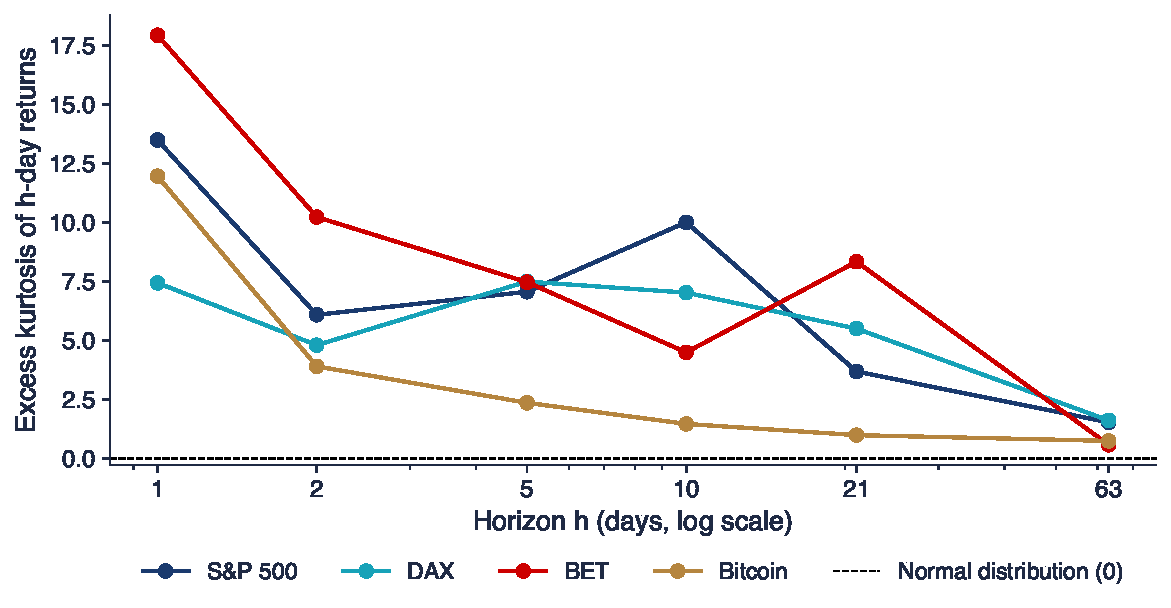
\includegraphics[width=0.97\textwidth,height=0.60\textheight,keepaspectratio]{sfm_ch2_aggregation.pdf}
\end{center}
\vspace{-0.25cm}
\begin{itemize}
    \item Excesul de aplatizare, zilnic $\to$ lunar $\to$ trimestrial: S\&P 500 13{,}5 $\to$ 3{,}7 $\to$ 1{,}5; BET 17{,}9 $\to$ 8{,}3 $\to$ 0{,}6; Bitcoin 12{,}0 $\to$ 1{,}0 $\to$ 0{,}7
    \item Scăderea este lentă și nemonotonă: o singură lună de crah (martie 2020) domină un eșantion de 200 de luni
    \item Randamentele trimestriale: JB nu mai respinge normalitatea pentru BET ($p = 0{,}07$) și Bitcoin ($p = 0{,}22$)
\end{itemize}
\sfmquantlet{Ch_02}{SFM_ch2_cont_stylised_facts}
\end{frame}

\begin{frame}{Faptul 2: S\&P 500, QQ plots pentru randamentele zilnice și lunare}
\itemsize{\footnotesize}
\begin{center}
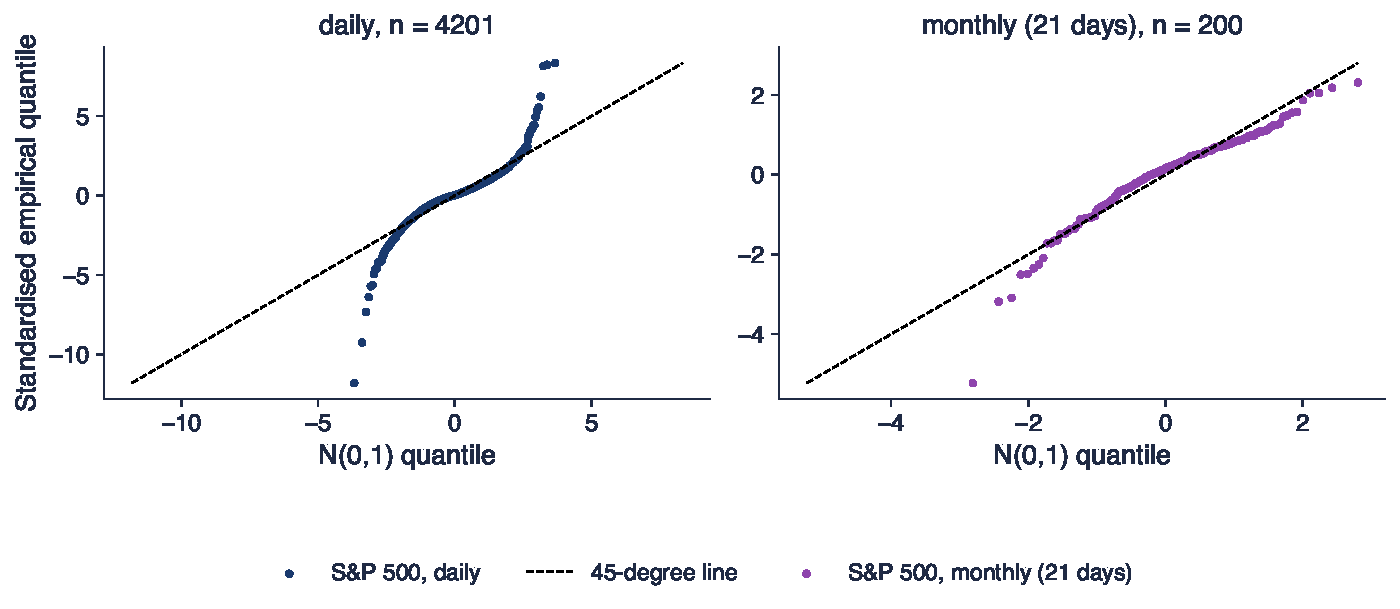
\includegraphics[width=0.97\textwidth,height=0.60\textheight,keepaspectratio]{sfm_ch2_qq_horizons.pdf}
\end{center}
\vspace{-0.25cm}
\begin{itemize}
    \item Randamentele lunare sînt mult mai aproape de dreaptă decît cele zilnice
    \item Dar randamentele lunare nu sînt Normale: asimetria $-1{,}18$, excesul de aplatizare $3{,}7$, $n = 200$; punctul cel mai de jos este martie 2020
    \item De ce atît de lent? Volatility clustering face randamentele zilnice dependente, ceea ce încetinește convergența din CLT
\end{itemize}
\sfmquantlet{Ch_02}{SFM_ch2_cont_stylised_facts}
\end{frame}

\begin{frame}{Faptul 3: absența autocorelației liniare}
\itemsize{\small}
\begin{itemize}
    \item \textbf{ACF} (autocorrelation function, funcția de autocorelație): $\rho(h) = \text{Corr}(r_t, r_{t-h})$, $h = 1, 2, \dots$
    \begin{itemize}
        \item versiunea de selecție $\hat\rho(h) = \sum_t (r_t - \bar r)(r_{t-h} - \bar r)/\sum_t (r_t - \bar r)^2$
        \item pentru date i.i.d., $\hat\rho(h) \approx N(0, 1/n)$: banda de 95\% $\pm 1{,}96/\sqrt{n}$
    \end{itemize}
    \item Testul \textbf{LB} (Ljung--Box) \refLB{} pentru $H_0$: $\rho(1) = \dots = \rho(m) = 0$
    \begin{itemize}
        \item $Q(m) = n(n+2)\sum_{h=1}^m \hat\rho(h)^2/(n - h) \sim \chi^2(m)$; pentru $m = 10$, respingem dacă $Q > 18{,}3$
    \end{itemize}
    \item De ce lipsește? Dacă randamentele ar fi previzibile, investitorii ar exploata acest lucru pînă cînd previzibilitatea dispare (piețe eficiente, \sfmchlink{https://danpele.github.io/SFM/RO/Cursuri/capitol7_piete_eficiente_mers_aleator_vr.pdf}{Capitolul 7})
\end{itemize}
\end{frame}

\begin{frame}{Faptele 3 și 4: ACF a randamentelor și a randamentelor absolute}
\itemsize{\footnotesize}
\begin{center}
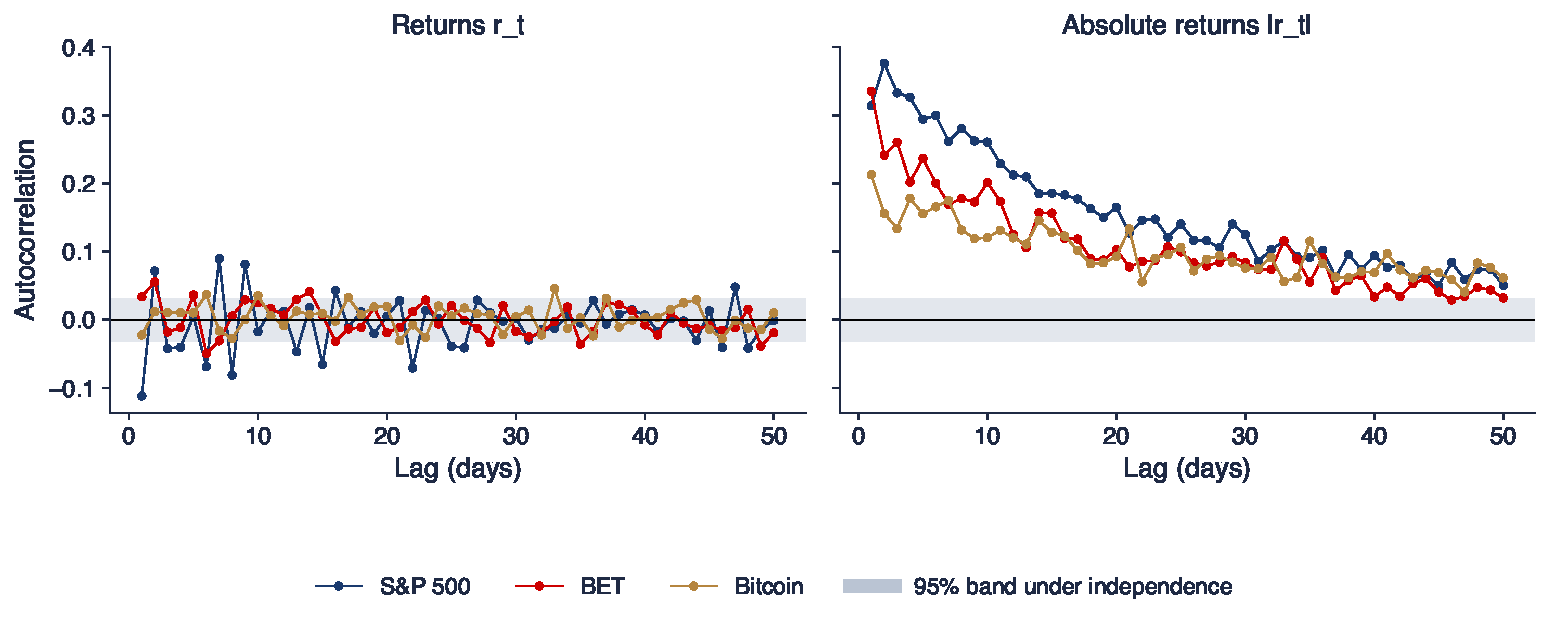
\includegraphics[width=0.97\textwidth,height=0.60\textheight,keepaspectratio]{sfm_ch2_acf.pdf}
\end{center}
\vspace{-0.25cm}
\begin{itemize}
    \item Stînga: randamentele; majoritatea autocorelațiilor sînt în bandă sau aproape de ea; S\&P 500 $\hat\rho(1) = -0{,}11$, BET $0{,}03$, Bitcoin $-0{,}02$
    \item Dreapta: randamentele absolute; toate pozitive, cu scădere lentă: S\&P 500 $0{,}31$ la decalajul 1, $0{,}26$ la decalajul 10, $0{,}05$ la decalajul 50
\end{itemize}
\sfmquantlet{Ch_02}{SFM_ch2_cont_stylised_facts}
\end{frame}

\begin{frame}{Faptul 3: autocorelație mică, dar nu întotdeauna nulă}
\itemsize{\small}
\begin{itemize}
    \item Ljung--Box $Q(10)$ pentru randamente: S\&P 500 199, BET 46, Bitcoin 20; valoarea critică 18{,}3
    \begin{itemize}
        \item formal, unele autocorelații sînt semnificative
    \end{itemize}
    \item Două motive pentru a nu supra-interpreta rezultatul
    \begin{itemize}
        \item valorile sînt mici din punct de vedere economic: $|\hat\rho(h)| \le 0{,}11$, deci se explică cel mult 1{,}2\% din varianță
        \item banda $\pm 1{,}96/\sqrt{n}$ presupune randamente i.i.d.; cu volatility clustering este prea îngustă, deci „semnificativ” apare prea des
    \end{itemize}
    \item Valoarea S\&P 500 la decalajul 1 provine mai ales din martie 2020, cînd căderile mari și revenirile au alternat: fără 20 februarie--30 aprilie 2020, $\hat\rho(1) = -0{,}04$
    \item Teste robuste ale previzibilității (testele raportului varianțelor): \sfmchlink{https://danpele.github.io/SFM/RO/Cursuri/capitol7_piete_eficiente_mers_aleator_vr.pdf}{Capitolul 7}
\end{itemize}
\end{frame}

\begin{frame}{Faptul 4: volatility clustering}
\itemsize{\footnotesize}
\begin{columns}[T]
\begin{column}{0.62\textwidth}
\begin{itemize}
    \item „Variațiile mari tind să fie urmate de variații mari, de orice semn, iar variațiile mici de variații mici” \refMandelbrot
    \item Semnul randamentului de mîine este imprevizibil; mărimea lui nu este
    \item Dovezi: ACF a lui $|r_t|$ pozitivă pe 50 de decalaje
    \begin{itemize}
        \item Ljung--Box $Q(10)$ pentru $|r_t|$: S\&P 500 3859, BET 2120, Bitcoin 1086
    \end{itemize}
    \item Deci randamentele sînt necorelate, dar \textbf{nu independente}
    \item Modele: ARCH și GARCH (Capitolul 9)
\end{itemize}
\end{column}
\begin{column}{0.34\textwidth}
\centering
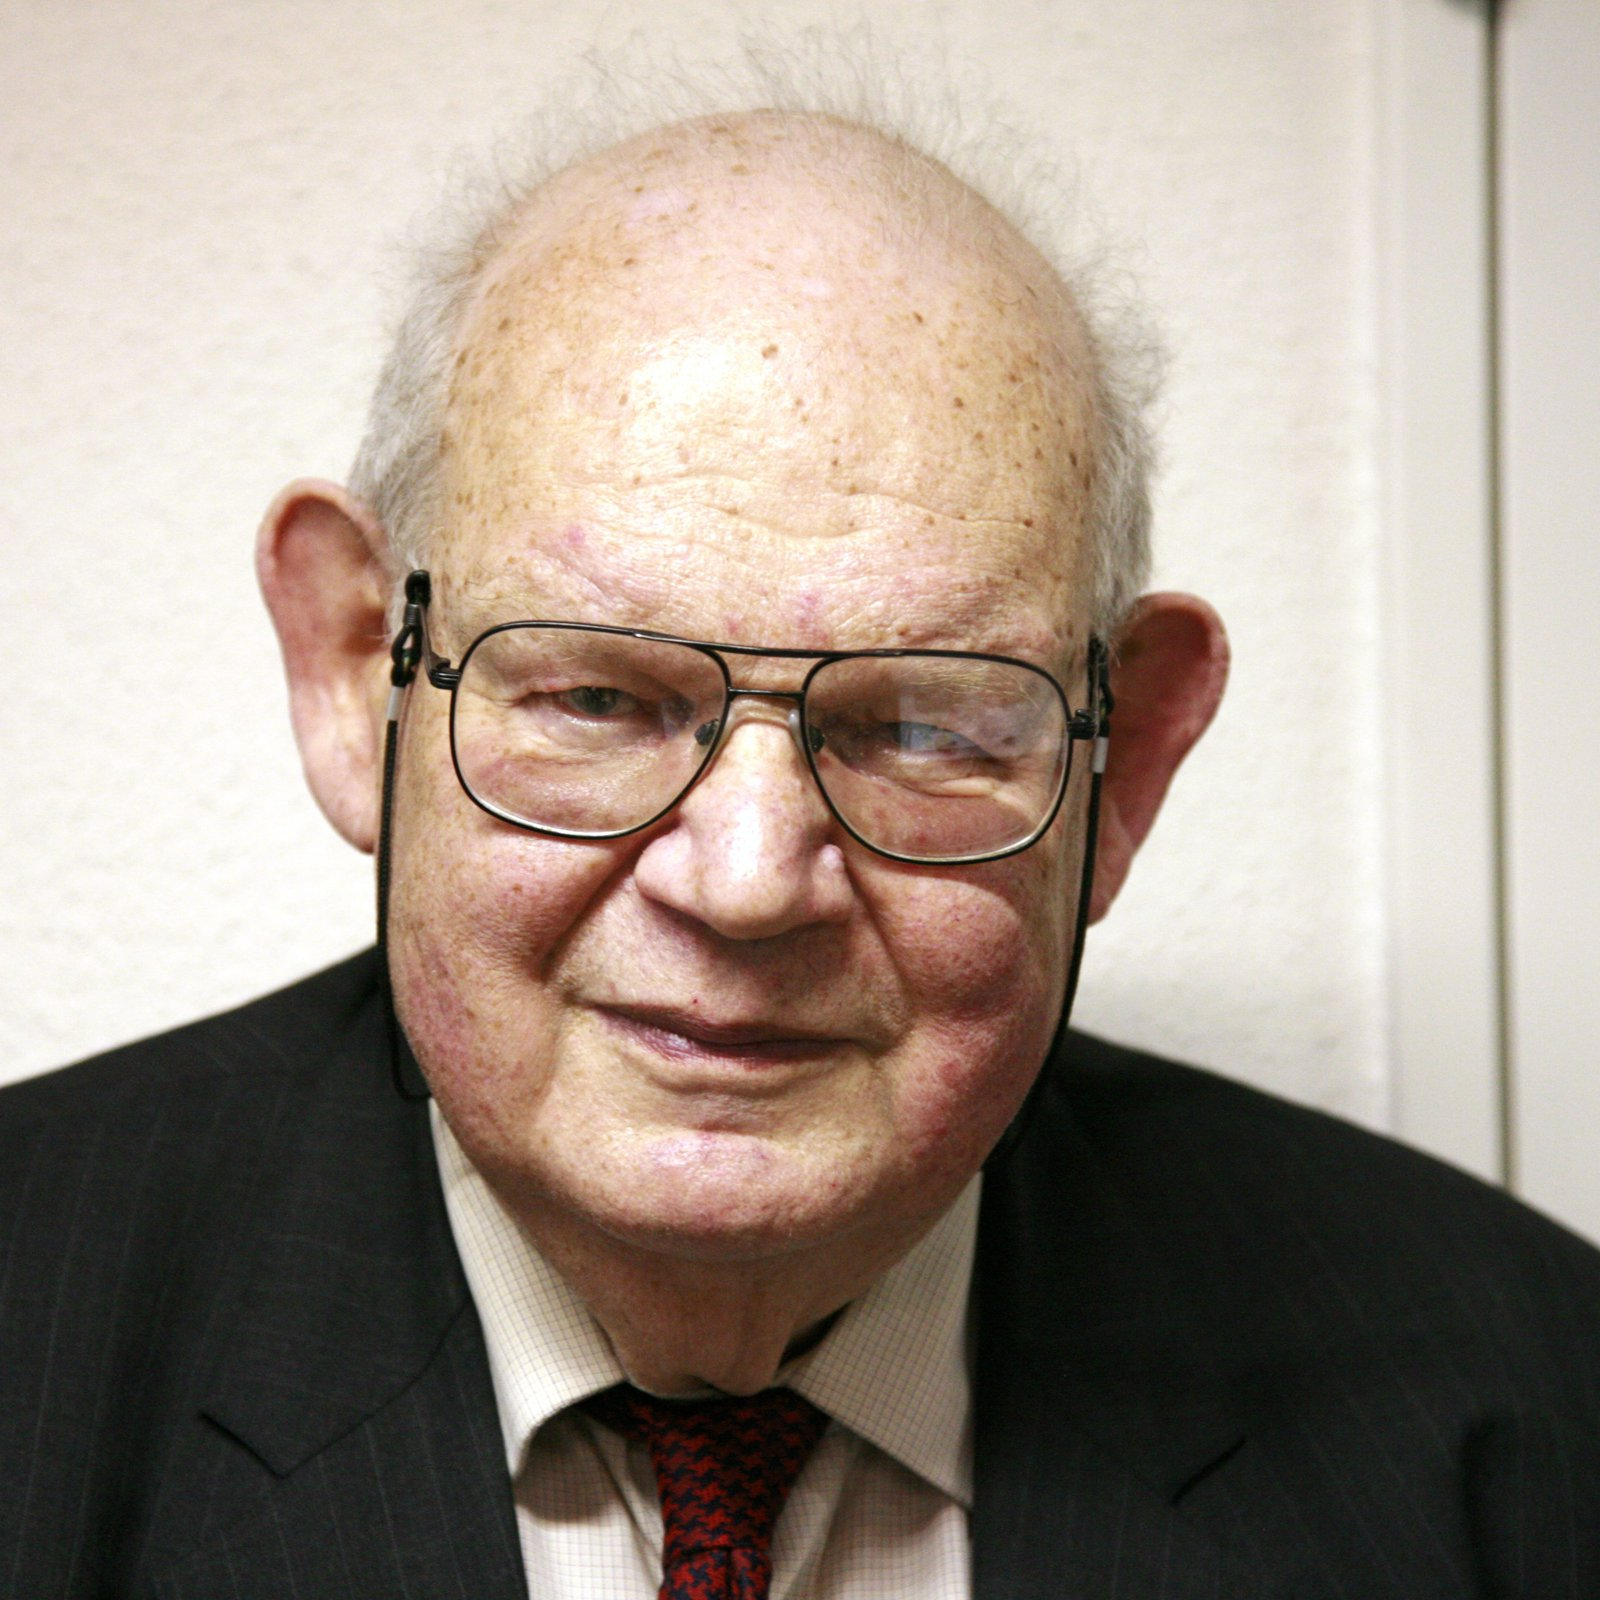
\includegraphics[height=0.42\textheight]{ch0_mandelbrot_2007.jpg}\\[1mm]
\imgcap{Benoit Mandelbrot (1924--2010)}
\imgcredit{https://commons.wikimedia.org/wiki/File:Benoit_Mandelbrot_mg_1804-d.jpg}{Foto: Rama (2007); CC BY-SA 2.0 fr; Wikimedia Commons}
\end{column}
\end{columns}
\end{frame}

\begin{frame}{Faptul 4: perioade calme și perioade agitate}
\itemsize{\footnotesize}
\begin{center}
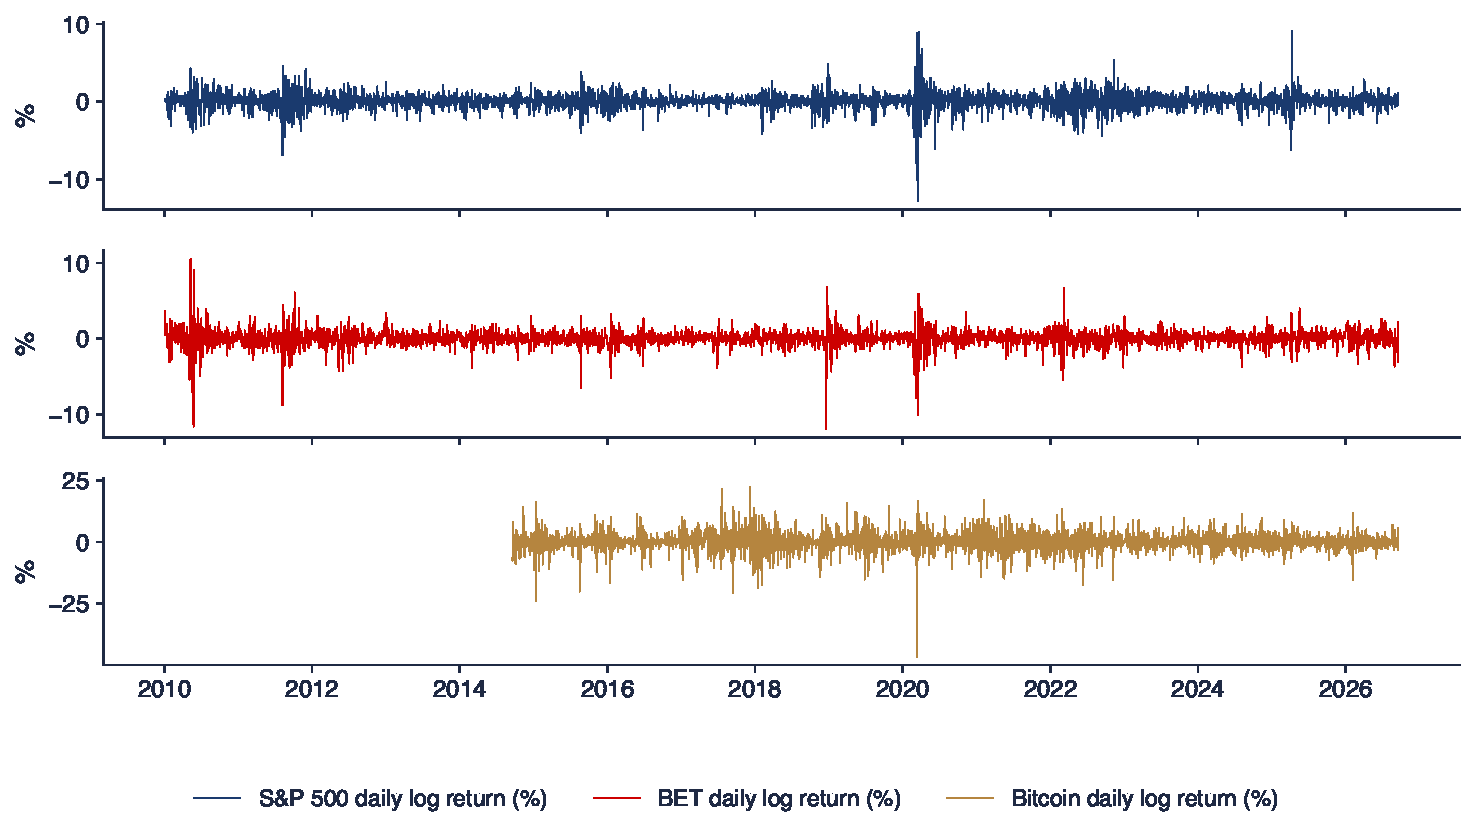
\includegraphics[width=0.97\textwidth,height=0.62\textheight,keepaspectratio]{sfm_ch2_clustering.pdf}
\end{center}
\vspace{-0.25cm}
\begin{itemize}
    \item Perioade agitate: 2010--2011 (criza datoriilor din zona euro), decembrie 2018 pentru BET, martie 2020 peste tot, aprilie 2025
    \item Între ele, ani calmi: volatilitatea unei zile depinde de perioada în care cade
\end{itemize}
\sfmquantlet{Ch_02}{SFM_ch2_cont_stylised_facts}
\end{frame}

\begin{frame}{Faptul 5: efectul de levier}
\itemsize{\small}
\begin{itemize}
    \item Măsura: $L(k) = \text{Corr}(r_t, |r_{t+k}|)$, $k = 1, 2, \dots$
    \begin{itemize}
        \item $L(k) < 0$: o scădere azi este urmată de mișcări mai mari decît o creștere de aceeași mărime
    \end{itemize}
    \item Explicația prin efectul de levier financiar \refChristie
    \begin{itemize}
        \item cînd prețul acțiunii scade, raportul datorii/capital propriu crește, deci capitalul propriu devine mai riscant
    \end{itemize}
    \item O a doua explicație, volatility feedback: o volatilitate așteptată mai mare mărește randamentul cerut și reduce prețurile
    \item Modele cu răspuns asimetric (EGARCH, GJR-GARCH): Capitolul 9
\end{itemize}
\end{frame}

\begin{frame}{Faptul 5: corelațiile de levier}
\itemsize{\footnotesize}
\begin{center}
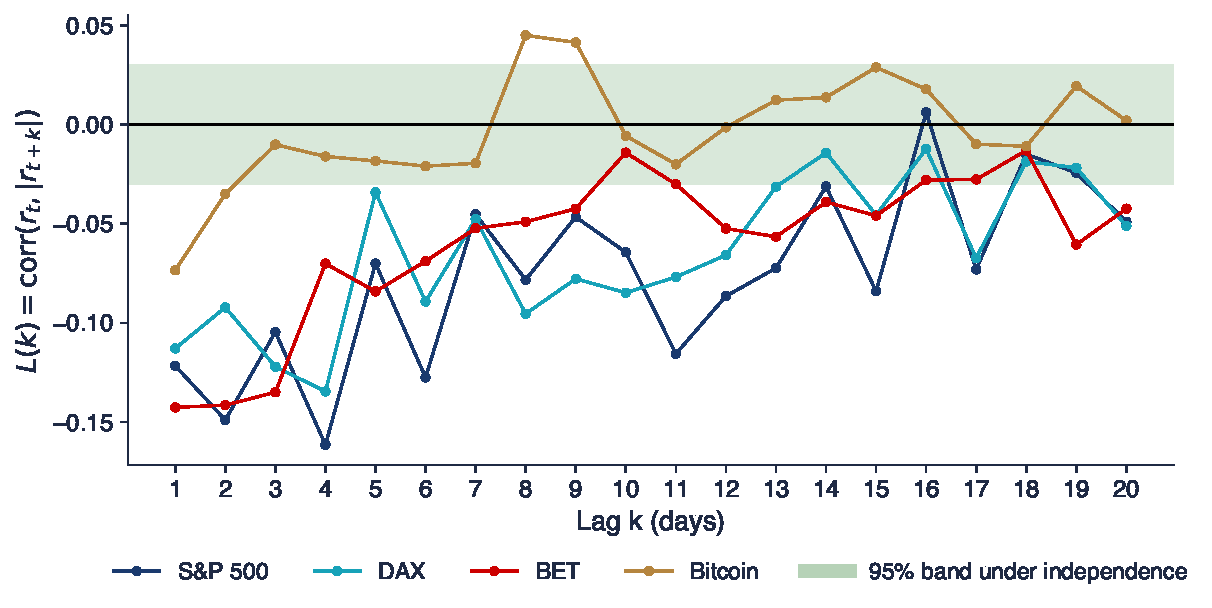
\includegraphics[width=0.97\textwidth,height=0.60\textheight,keepaspectratio]{sfm_ch2_leverage.pdf}
\end{center}
\vspace{-0.25cm}
\begin{itemize}
    \item Indicii bursieri: $L(k) < 0$ pentru majoritatea primelor 20 de decalaje; media $L(1..5)$: S\&P 500 $-0{,}12$, DAX $-0{,}10$, BET $-0{,}11$
    \item Bitcoin: $L(1) = -0{,}07$, apoi în interiorul benzii: în spatele Bitcoin nu există o firmă cu datorii, deci mecanismul de levier lipsește
\end{itemize}
\sfmquantlet{Ch_02}{SFM_ch2_cont_stylised_facts}
\end{frame}

\begin{frame}{Faptul 6: asimetria cîștig/pierdere}
\itemsize{\footnotesize}
\begin{center}
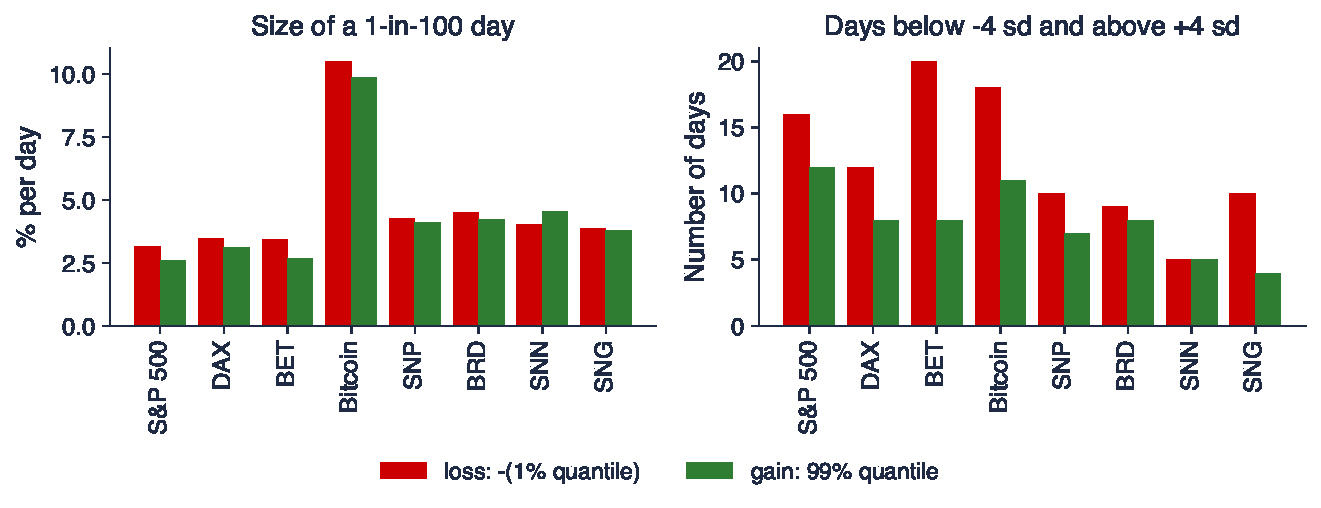
\includegraphics[width=0.97\textwidth,height=0.60\textheight,keepaspectratio]{sfm_ch2_gain_loss.pdf}
\end{center}
\vspace{-0.25cm}
\begin{itemize}
    \item Stînga: la indici, pierderea depășită într-o zi din 100 este mai mare decît cîștigul depășit într-o zi din 100: BET 3{,}45\% față de 2{,}66\%, S\&P 500 3{,}15\% față de 2{,}61\%
    \item Dreapta: zile sub $-4\sigma$ față de peste $+4\sigma$: BET 20 față de 8, S\&P 500 16 față de 12, Bitcoin 18 față de 11
    \item Excepție: SNN, cu asimetrie pozitivă și cuantila din dreapta mai mare
\end{itemize}
\sfmquantlet{Ch_02}{SFM_ch2_sigma_days}
\end{frame}

\begin{frame}{Șase fapte, opt serii}
\itemsize{\footnotesize}
\begin{center}
\scriptsize
\begin{tabular}{lrrrrrr}
\toprule
Seria & Exces apl. & Exces apl., 21 de zile & $\hat\rho_r(1)$ & $\hat\rho_{|r|}(10)$ & $\bar L(1..5)$ & $|q_{0{,}01}|/q_{0{,}99}$ \\
\midrule
S\&P 500 & $13{,}5$ & $3{,}7$ & $-0{,}11$ & $0{,}26$ & $-0{,}12$ & $1{,}21$ \\
DAX & $7{,}4$ & $5{,}5$ & $0{,}01$ & $0{,}16$ & $-0{,}10$ & $1{,}12$ \\
BET & $17{,}9$ & $8{,}3$ & $0{,}03$ & $0{,}20$ & $-0{,}11$ & $1{,}30$ \\
Bitcoin & $12{,}0$ & $1{,}0$ & $-0{,}02$ & $0{,}12$ & $-0{,}03$ & $1{,}07$ \\
OMV Petrom (SNP) & $8{,}9$ & $3{,}3$ & $-0{,}02$ & $0{,}13$ & $-0{,}03$ & $1{,}04$ \\
BRD & $7{,}3$ & $0{,}4$ & $0{,}03$ & $0{,}11$ & $-0{,}05$ & $1{,}07$ \\
Nuclearelectrica (SNN) & $5{,}1$ & $2{,}3$ & $0{,}09$ & $0{,}08$ & $-0{,}03$ & $0{,}88$ \\
Romgaz (SNG) & $5{,}3$ & $1{,}4$ & $0{,}07$ & $0{,}08$ & $-0{,}04$ & $1{,}02$ \\
\bottomrule
\end{tabular}
\end{center}
\begin{itemize}
    \item Faptele 1, 3 și 4 sînt valabile pentru toate seriile; faptul 2, cu estimări imprecise; faptele 5 și 6, pentru indici și majoritatea acțiunilor BVB, slab sau deloc pentru Bitcoin și SNN
    \item O comparație între distribuțiile randamentelor criptomonedelor și cele ale activelor tradiționale: \refPeleCrypto
\end{itemize}\sfmquantlet{Ch_02}{SFM_ch2_cont_stylised_facts}
\end{frame}

\begin{frame}{Implicațiile faptelor stilizate pentru modele}
\itemsize{\small}
\begin{center}
\footnotesize
\begin{tabular}{lcccccc}
\toprule
Model & 1 & 2 & 3 & 4 & 5 & 6 \\
\midrule
i.i.d. Normal & -- & trivial & \checkmark & -- & -- & -- \\
i.i.d. Student-$t$ & \checkmark & \checkmark & \checkmark & -- & -- & -- \\
GARCH cu erori $t$ (cap.~9) & \checkmark & \checkmark & \checkmark & \checkmark & -- & -- \\
EGARCH, GJR-GARCH (cap.~9) & \checkmark & \checkmark & \checkmark & \checkmark & \checkmark & (\checkmark) \\
\bottomrule
\end{tabular}
\end{center}
\begin{itemize}
    \item Coloanele: cele șase fapte în ordinea din această secțiune; (\checkmark): doar pentru randamente pe mai multe zile, dacă erorile nu sînt asimetrice
    \item Măsurile de risc (VaR 1\%, ES 2,5\%, Capitolul 10) moștenesc calitatea modelului: un VaR Normal este prea mic în crize
    \item O măsură înrudită a riscului de coadă, entropia informațională: \refPeleEntropy
\end{itemize}
\end{frame}

\begin{frame}{Recapitulare: fapte stilizate}
\itemsize{\small}
\begin{itemize}
    \item Cozi groase: o zi de 4 sigma la fiecare cîteva luni, în loc de una la cîteva decenii
    \item Randamentele sînt aproape necorelate, dar mărimea lor este puternic autocorelată
    \item Pe orizonturi mai lungi, randamentele se apropie lent de distribuția Normală
    \item Indicii bursieri: scăderile cresc volatilitatea, iar pierderile sînt mai mari decît cîștigurile
\end{itemize}
\end{frame}


%=============================================================================
\section{AI pentru descoperire științifică}
%=============================================================================

\begin{frame}{O întrebare deschisă: devin mai subțiri cozile Bitcoin?}
\itemsize{\footnotesize}
\begin{columns}[T]
\begin{column}{0.52\textwidth}
\begin{center}
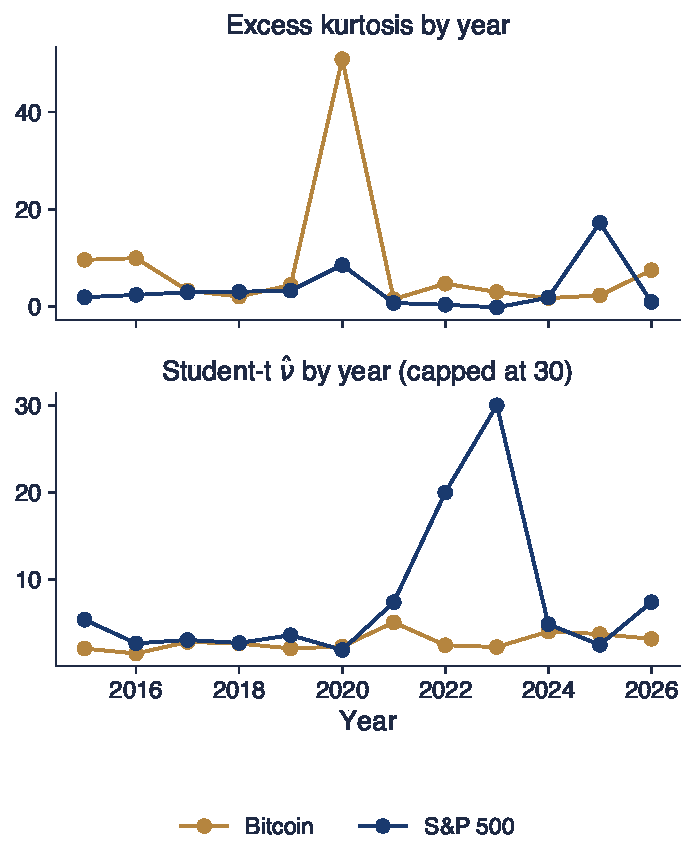
\includegraphics[width=\linewidth,height=0.78\textheight,keepaspectratio]{sfm_ch2_tails_by_year.pdf}
\end{center}
\end{column}
\begin{column}{0.44\textwidth}
\begin{itemize}
    \item Pe măsură ce o piață se maturizează (mai mulți participanți, futures, ETF-uri), cozile ei s-ar putea subția
    \item Bitcoin, 2015--2026: $\hat\nu$ anual între 1{,}5 și 5{,}1; corelația rangurilor cu anul $0{,}63$ ($p = 0{,}03$)
    \item De ce rămîne deschisă: 12 estimări anuale imprecise, un an (2020, exces de aplatizare 51) dominat de o singură zi
    \item Instrumentele AI pot accelera un astfel de studiu; nu înlocuiesc verificarea lui \refWang
\end{itemize}
\end{column}
\end{columns}
\sfmquantlet{Ch_02}{SFM_ch2_tails_by_year}
\end{frame}

\begin{frame}{Contribuția posibilă a AI}
\itemsize{\small}
\begin{itemize}
    \item \textbf{Literatura}: găsirea studiilor despre indicii de coadă ai activelor cripto și rezumarea metodelor lor
    \item \textbf{Cod}: o primă versiune a estimărilor pe ferestre mobile pentru $\nu$ și excesul de aplatizare
    \item \textbf{Robustețe}: propunerea altor ferestre, altor măsuri ale cozilor (\sfmchlink{https://danpele.github.io/SFM/RO/Cursuri/capitol5_cozi_groase_evt.pdf}{Capitolul 5}), altor active cripto
    \item Exemplu de prompt
    \begin{itemize}
        \item \aiprompt{Write a Python function that fits a Student-t distribution to daily Bitcoin log returns on rolling 365-day windows and returns the degrees of freedom with a bootstrap 95\% interval.}
    \end{itemize}
\end{itemize}
\end{frame}

\begin{frame}{Verificări necesare}
\itemsize{\small}
\begin{itemize}
    \item Datele: aceeași coloană de preț și același calendar pentru fiecare an; erori printre cele mai mari mișcări
    \item Estimarea: a convers optimizatorul? $\hat\nu$ aproape de 2 sau peste 30 trebuie reverificat
    \item Inferența: o singură estimare $\hat\nu$ pe an este imprecisă; raportați intervale, nu doar estimări punctuale
    \item Volatility clustering: cozi anuale mai subțiri pot însemna doar ani mai calmi (Capitolul 9)
    \item Referințele: fiecare lucrare citată trebuie să existe; verificați DOI-ul
\end{itemize}
\end{frame}

\begin{frame}{Idee de proiect}
\itemsize{\small}
\begin{itemize}
    \item \textbf{Întrebarea}: se subțiază cozile activelor cripto pe măsură ce piețele lor se maturizează?
    \begin{itemize}
        \item date: Bitcoin, Ethereum și Solana din datele cursului; S\&P 500 ca reper
    \end{itemize}
    \item Pași
    \begin{itemize}
        \item estimați $\hat\nu$ și excesul de aplatizare pe ferestre mobile de un an, cu intervale bootstrap
        \item testați existența unui trend; repetați pe randamente împărțite la o volatilitate mobilă
        \item comparați numărul zilelor de 4 sigma pe an cu S\&P 500
    \end{itemize}
    \item Rezultat: un tabel, un grafic și un paragraf despre ce pot și ce nu pot arăta datele
    \item Declarați orice folosire a AI și listați erorile AI pe care le-ați corectat
\end{itemize}
\end{frame}


%=============================================================================
\section{Rezumat}
%=============================================================================

\begin{frame}{Idei principale}
\itemsize{\small}
\begin{itemize}
    \item Distribuția Normală: doi parametri, cozi subțiri, închisă la adunare
    \item Randamentele logaritmice Normale dau prețuri lognormale; media depășește mediana prin volatility drag
    \item CLT cere independență, distribuție identică și varianță finită
    \item Randamentele zilnice: în general asimetrie negativă, exces de aplatizare 5--18, JB respinge, QQ plots se curbează la ambele capete
    \item Student-$t$ cu $\hat\nu$ între 2 și 5 descrie mult mai bine cozile, dar este simetrică și i.i.d.
    \item Șase fapte stilizate: cozi groase, gaussianitate agregată, fără autocorelație liniară, volatility clustering, efect de levier, asimetrie cîștig/pierdere
\end{itemize}
\end{frame}

\begin{frame}{Formule de reținut}
\itemsize{\small}
\begin{center}
\footnotesize
\begin{tabular}{ll}
\toprule
\textbf{Mărimea} & \textbf{Formula} \\
\midrule
Densitatea Normală & $f(x) = (\sigma\sqrt{2\pi})^{-1}\exp\big(-(x - \mu)^2/(2\sigma^2)\big)$ \\
Momentele lognormale & mediana $e^m$, media $e^{m + s^2/2}$ \\
CLT & $\sqrt{n}(\bar X_n - \mu)/\sigma \xrightarrow{d} N(0,1)$ \\
Asimetria, excesul de aplatizare & $S = m_3/m_2^{3/2}$, \quad $K = m_4/m_2^2 - 3$ \\
Jarque--Bera & $\text{JB} = \frac{n}{6}(S^2 + K^2/4) \sim \chi^2(2)$ \\
Student-$t(\nu)$ & varianța $\nu/(\nu - 2)$, excesul de aplatizare $6/(\nu - 4)$ \\
AIC & $2k - 2\ell$ \\
ACF, Ljung--Box & $\hat\rho(h)$, \quad $Q(m) = n(n+2)\sum_{h=1}^m \hat\rho(h)^2/(n - h)$ \\
Levier & $L(k) = \text{Corr}(r_t, |r_{t+k}|)$ \\
\bottomrule
\end{tabular}
\end{center}
\end{frame}

\begin{frame}{Verificați-vă}
\itemsize{\small}
\begin{itemize}
    \item \textbf{Întrebare}: randamentele zilnice sînt $N(0{,}05\%, 1\%^2)$; la cîte abateri standard se află o zi de $-3\%$?
    \begin{itemize}
        \item \textbf{Răspuns}: $z = (-3 - 0{,}05)/1 = -3{,}05$
    \end{itemize}
    \item \textbf{Întrebare}: $n = 2500$, $S = -0{,}5$, $K = 6$; cît este JB?
    \begin{itemize}
        \item \textbf{Răspuns}: $\frac{2500}{6}(0{,}25 + 9) = 3854$; normalitatea este respinsă
    \end{itemize}
    \item \textbf{Întrebare}: un randament logaritmic anual este $N(5\%, 20\%^2)$; care sînt mediana și media valorii unei investiții de 100 după un an?
    \begin{itemize}
        \item \textbf{Răspuns}: mediana $100e^{0{,}05} = 105{,}1$, media $100e^{0{,}05 + 0{,}02} = 107{,}3$
    \end{itemize}
    \item Urmează: \sfmchlink{https://danpele.github.io/SFM/RO/Cursuri/capitol3_distributii_alfa_stabile.pdf}{Capitolul 3}, distribuții $\alpha$-stabile
\end{itemize}
\end{frame}


%=============================================================================
\section{Bibliografie}
%=============================================================================

\begin{frame}{Bibliografie (1/2)}
\itemsize{\tiny}
\begin{itemize}
    \item Akaike, H. (1974). \href{https://doi.org/10.1109/TAC.1974.1100705}{A new look at the statistical model identification}. \textit{IEEE Transactions on Automatic Control}, 19(6), 716--723.
    \item Bachelier, L. (1900). \href{https://doi.org/10.24033/asens.476}{Théorie de la spéculation}. \textit{Annales scientifiques de l'École Normale Supérieure}, 17, 21--86.
    \item Blattberg, R.C., Gonedes, N.J. (1974). \href{https://doi.org/10.1086/295634}{A comparison of the stable and Student distributions as statistical models for stock prices}. \textit{Journal of Business}, 47(2), 244--280.
    \item Bollerslev, T. (1987). \href{https://doi.org/10.2307/1925546}{A conditionally heteroskedastic time series model for speculative prices and rates of return}. \textit{Review of Economics and Statistics}, 69(3), 542--547.
    \item Borak, S., Härdle, W.K., López-Cabrera, B. (2013). \href{https://doi.org/10.1007/978-3-642-33929-5}{\textit{Statistics of Financial Markets: Exercises and Solutions}}, 2nd ed. Springer.
    \item Christie, A.A. (1982). \href{https://doi.org/10.1016/0304-405X(82)90018-6}{The stochastic behavior of common stock variances: value, leverage and interest rate effects}. \textit{Journal of Financial Economics}, 10(4), 407--432.
    \item Cont, R. (2001). \href{https://doi.org/10.1080/713665670}{Empirical properties of asset returns: stylized facts and statistical issues}. \textit{Quantitative Finance}, 1(2), 223--236.
    \item Fama, E.F. (1965). \href{https://doi.org/10.1086/294743}{The behavior of stock-market prices}. \textit{Journal of Business}, 38(1), 34--105.
    \item Franke, J., Härdle, W.K., Hafner, C.M. (2019). \href{https://doi.org/10.1007/978-3-030-13751-9}{\textit{Statistics of Financial Markets: An Introduction}}, 5th ed. Springer.
    \item Jarque, C.M., Bera, A.K. (1980). \href{https://doi.org/10.1016/0165-1765(80)90024-5}{Efficient tests for normality, homoscedasticity and serial independence of regression residuals}. \textit{Economics Letters}, 6(3), 255--259.
    \item Jarque, C.M., Bera, A.K. (1987). \href{https://doi.org/10.2307/1403192}{A test for normality of observations and regression residuals}. \textit{International Statistical Review}, 55(2), 163--172.
\end{itemize}
\end{frame}

\begin{frame}{Bibliografie (2/2)}
\itemsize{\tiny}
\begin{itemize}
    \item Ljung, G.M., Box, G.E.P. (1978). \href{https://doi.org/10.1093/biomet/65.2.297}{On a measure of lack of fit in time series models}. \textit{Biometrika}, 65(2), 297--303.
    \item Mandelbrot, B. (1963). \href{https://doi.org/10.1086/294632}{The variation of certain speculative prices}. \textit{Journal of Business}, 36(4), 394--419.
    \item Osborne, M.F.M. (1959). \href{https://doi.org/10.1287/opre.7.2.145}{Brownian motion in the stock market}. \textit{Operations Research}, 7(2), 145--173.
    \item Pele, D.T., Lazar, E., Dufour, A. (2017). \href{https://doi.org/10.3390/e19050226}{Information entropy and measures of market risk}. \textit{Entropy}, 19(5), 226.
    \item Pele, D.T., Wesselhöfft, N., Härdle, W.K., Kolossiatis, M., Yatracos, Y.G. (2023). \href{https://doi.org/10.1080/1351847X.2021.1960403}{Are cryptos becoming alternative assets?} \textit{European Journal of Finance}, 29(10), 1064--1105.
    \item Praetz, P.D. (1972). \href{https://doi.org/10.1086/295425}{The distribution of share price changes}. \textit{Journal of Business}, 45(1), 49--55.
    \item Student (1908). \href{https://doi.org/10.1093/biomet/6.1.1}{The probable error of a mean}. \textit{Biometrika}, 6(1), 1--25.
    \item Tsay, R.S. (2010). \href{https://doi.org/10.1002/9780470644560}{\textit{Analysis of Financial Time Series}}, 3rd ed. Wiley.
    \item Wang, H., Fu, T., Du, Y., Gao, W., et al. (2023). \href{https://doi.org/10.1038/s41586-023-06221-2}{Scientific discovery in the age of artificial intelligence}. \textit{Nature}, 620, 47--60.
    \item Wilk, M.B., Gnanadesikan, R. (1968). \href{https://doi.org/10.1093/biomet/55.1.1}{Probability plotting methods for the analysis of data}. \textit{Biometrika}, 55(1), 1--17.
\end{itemize}
\end{frame}

\end{document}
